\documentclass[12pt]{article}
\usepackage{amssymb,amsmath,natbib,graphicx,amsthm,
  setspace,sectsty,anysize,times,dsfont,enumerate}

\usepackage[svgnames]{xcolor}

\usepackage{lscape,arydshln,relsize,rotating,multirow}
\usepackage{caption}
\captionsetup{%
  font=small,
  labelfont=normalfont,
  singlelinecheck=false,
  justification=justified
}
\usepackage{algorithm}

\newtheorem{prop}{\sc Proposition}[section]
\newtheorem{theorem}{\sc Theorem}[section]
\newtheorem{definition}{\sc Definition}[section]
\newtheorem{lemma}{\sc Lemma}[section]
\newtheorem{corollary}{\sc Corollary}[section]

\marginsize{1.1in}{.9in}{.3in}{1.4in}

\newcommand{\nb}{\color{blue}}
\newcommand{\dbl}{\setstretch{1.5}}
\newcommand{\sgl}{\setstretch{1.1}}

\newcommand{\bs}[1]{\boldsymbol{#1}}
\newcommand{\mc}[1]{\mathcal{#1}}
\newcommand{\mr}[1]{\mathrm{#1}}
\newcommand{\bm}[1]{\mathbf{#1}}
\newcommand{\ds}[1]{\mathds{#1}}
\newcommand{\indep}{\perp\!\!\!\perp}
\DeclareMathOperator*{\argmin}{argmin}
\newcommand{\norm}[1]{|\!|#1|\!|_{1}}
\newcommand{\code}[1]{{\smaller\sf#1}}
\newcommand{\e}[1]{{\footnotesize$\times10$}{$^{#1}$}}

\sectionfont{\noindent\normalfont\large\bf}
\subsectionfont{\noindent\normalfont\normalsize\bf}
\subsubsectionfont{\noindent\normalfont\it}

\usepackage[bottom,hang,flushmargin]{footmisc}

\pdfminorversion=4
\begin{document}

\sgl 

\pagestyle{empty}

~
\vskip 3cm

\noindent {\huge \bf The Gamma Lasso} 

\vskip 1cm

\noindent{\Large Matt Taddy}

{\large
\vskip .5cm \noindent
{The  University of Chicago Booth School of Business}\\
{\tt faculty.chicagobooth.edu/matt.taddy}}



\vskip 2cm

{\noindent This article describes a very fast algorithm for obtaining
continuous regularization paths corresponding to cost functions spanning the
range of concavity between $L_0$ and $L_1$ norms.  The `gamma lasso' heuristic
does $L_1$ (lasso) penalized regression estimation on a grid of decreasing
penalties, but adapts coefficient-specific weights to decrease as a function
of the estimated coefficient in the previous path segment.  Our particular
weight-updating scheme is motivated from a Bayesian model, and is related to
estimation under log penalties.  This very simple recipe is used to illustrate
the large and difficult literature on concave penalization, with the hope that
we can make the ideas more accessible to practitioners. The construction also
leads us to a plug-in estimator for degrees of freedom; this is applied in
model selection, and in experimentation our  information criteria 
perform as well as cross-validation. The work is illustrated in linear
regression simulations and in application of logistic regression to evaluate
 hockey players.}
 

\newpage
\dbl

\pagestyle{plain}
\vskip 1cm
\section{Introduction}
\label{intro}

For regression in high-dimensions it is useful to regularize estimation with a
penalty on coefficient size.  One minimizes the negative log
likelihood plus a sum of cost functions applied to each coefficient's distance
from zero.  When these cost functions have a non-differentiable spike at zero,
the optimal solution can be sparse.   The curvature of the penalty away from
zero dictates the weight of shrinkage imposed on the nonzero coefficients:
zero curvature is an $L_1$ penalty, as used in the common lasso regression
framework \citep{tibshirani_regression_1996}, and as curvature goes towards
$-\infty$ one approaches the $L_0$ penalty of subset selection.

Imagine that you are a data analyst familiar with classical methods, such as
hypothesis testing,  looking to try some of these more modern sparse
regularized regression techniques.  Strictly concave penalties, with negative
curvature instead of lasso's zero second derivative,  are tempting because
they provide near-unbiased estimation for large signals.  That is, if
$\hat\beta_j\neq0$ then it will be close to the result for  maximum likelihood
estimation (MLE) on {\it in-the-model} coefficients. Unfortunately, you will
discover that computation is difficult with these strictly concave penalties.
Most available software takes far longer to run than convex
alternatives and the solvers are not generally globally convergent.  At the
extreme, solving for $L_0$ regularized coefficients is NP hard. In contrast,
the lasso has a very fast forward stepwise procedure \citep{efron_least_2004},
easy-to-estimate degrees of freedom \citep{zou_degrees_2007}, and is far more
widely used in practice. These conveniences are due to the estimator stability
that results from lasso's nondiminishing bias. How do you decide what to use,
and is it possible to quickly evaluate the range of options between $L_0$ and
$L_1$ costs?

We introduce in Section \ref{glsec} the `gamma lasso' (GL) algorithm.  The
purpose of the article is then twofold. First, to advertise a very fast and
stable estimation framework that inherits many of the desirable properties of
concave penalized estimation: algorithm details are in Section
\ref{implement}, simple Monte-Carlo and information criterion model selection
are in Section \ref{selection},  and all methods are implemented in the {\tt gamlr}
package for {\sf R}.  Second, by reading the large and difficult literature on
concave regularization   in the context of our simple algorithm, we seek to
provide an intuitive overview on practical application of these techniques.
This includes Bayesian interpretations in Section \ref{bayes}, consistency and
unbiasedness properties in Section \ref{concave}, types and benefits of
estimator stability in Section \ref{stability}, available estimation routines
in Section \ref{lla}, and model complexity (degrees of freedom) in Section
\ref{dof}.

This mixture of goals follows from our personal use of the GL routine, both as
a workhorse in applications and as a tool for explaining non-convex penalized
estimation to non-experts.  The ideas are illustrated via linear regression
simulations in Section \ref{sim} and in logistic regression to evaluate
the ability of hockey players in Section \ref{nhl}. Section \ref{discussion}
closes with a brief discussion.

\section{The gamma lasso}
\label{glsec}

Denote the data matrix of $p$ covariates for $n$ observations as $\bm{X} =
[\bm{x}_1 \cdots \bm{x}_n]'$, where $\bm{x}_i = [x_{i1},\ldots,x_{ip}]'$, and
the associated response as $\bm{y} = [y_1,\ldots,y_n]'$. Write $\bs{x}_j = [x_{1j},\ldots,x_{nj}]'$ for the $j^{th}$ column of the design matrix $\bm{X}$.  Since the size of penalized $\beta_j$ depends upon the units of $x_{ij}$,  it is common to scale
the coefficient by $\mr{sd}_j$, the standard deviation of the $j^{th}$ column
of $\bm{X}$; this is achieved if $x_{ij}$ is replaced by $x_{ij}/\mr{sd}_j$
throughout. Write $\eta_{i} =
\alpha+\bm{x}_i'\bs{\beta}$ as the linear equation for observation $i$, and
denote with $l(\alpha, \bs{\beta}) = l(\bs{\eta})$  an unregularized
objective  proportional to the negative log likelihood.  In Gaussian (linear)
regression with independent normal errors, $l(\bs{\eta})$ is the sum-of-
squares $0.5\sum_i \left(y_i - \eta_i\right)^2$ and in binomial (logistic)
regression,  $l(\bs{\eta}) = -\sum_i \left[\eta_iy_i -
\log(1+e^{\eta_i})\right]$ for $y_i \in [0,1]$.  

The gamma lasso in Algorithm \ref{gammalasso}, for `scale' $\gamma \geq 0$,
yields paths of penalized coefficient estimates $\bs{\hat\beta}^1 \ldots
\bs{\hat\beta}^T$ (and intercepts $\hat\alpha^1 \ldots \hat\alpha^T$)
corresponding to $L_1$ penalties $\lambda^1 > \lambda^2 \ldots > \lambda^T$
multiplied against adaptive coefficient-specific weight adjustments
$\bs{\omega}^1 \ldots \bs{\omega}^T$.

\vskip .25cm
\begin{algorithm}[ht]
\caption{\label{gammalasso} The gamma lasso }
\vskip .25cm
Initialize $\bs{\omega}^1 = \bf{1}$ and $\lambda^1 >
0$ with step size
$0 < \delta < 1$.

\vspace{-.75cm}
\begin{align}
\text{for}~t=1\ldots T :&\notag \\
\left[\hat\alpha,\bs{\hat\beta}\right]^t &= \argmin_{\alpha,\beta_j\in\ds{R}}~~
l(\alpha,\bs{\beta}) + n\sum_j \lambda^t\omega^t_j|\beta_j| \label{l1pen}\\
\omega^{t+1}_j  &= \left(1 + \gamma |\hat\beta^t_j|\right)^{-1} ~~j=1\ldots p \label{adjweight}\\
\lambda^{t+1} &= \delta \lambda^t\notag
\end{align}
\end{algorithm}


Outputs from this type of algorithm -- a $p \times T$
field of $\bs{\hat\beta}$ estimates obtained while moving from high to low
penalization -- are referred to as {\it regularization paths}.  LARS
\citep{efron_least_2004} is a well-known example.  
The approach is nice not only because it leads to a full range of candidates
for model selection (as in Section
\ref{selection}), but also because $\bs{\hat\beta}^t$ at $\lambda^t$
provide {\it hot-starts} for $\bs{\hat\beta}^{t+1}$ at the next penalty level.
If the paths are near continuous (see Section \ref{stability}), estimation
over the full path can be faster than cold-start solution for a single penalty
specification.


To start such paths, $\lambda^1$ is commonly set to infimum $\lambda$ such
that (\ref{l1pen}) is minimized at $\bs{\hat\beta} = \bm{0}$.  Write
$g_j(\bs{\hat\beta})$ for the $j^{th}$ coefficient gradient of
$l(\alpha,\bs{\beta})$ (see \ref{models}) evaluated at
estimates  $[\hat \alpha, \bs{\hat \beta}]$, where it is implied that
$\hat\alpha$ has been set to minimize $l(\alpha,\bs{\hat\beta})$. The initial
value is  available analytically as 
\begin{equation}\label{maxabsgrad}
\lambda^1 = n^{-1}\max\{|g_j(\bm{0})|,~j=1\ldots p\},
\end{equation}
the maximum mean absolute gradient for the
null model with $\bs{\beta} = \bm{0}$. Given a path-length $T$, $\lambda^T$ is
 specified as a ratio of $\lambda^1$ (e.g., $\lambda^T = 0.01\lambda^1$)
and the step-size $\delta$ is implied as a consequence.

Behavior of the GL paths along a given $\bs{\lambda}$ sequence is governed by
$\gamma$, which we refer to as the penalty scale (see Section
\ref{bayes}).  Under $\gamma=0$ the weights are $\omega_j^t = 1$ for all $j,t$
and Algorithm \ref{gammalasso} is just the usual lasso.  At the other extreme,
$\gamma=\infty$ yields a subset selection routine where a coefficient is
unpenalized in all segments after it first becomes nonzero. Figure
\ref{gamlr_eg} shows solutions as a function of $\lambda^t$ in a simple
problem. Moving from the lasso ($\gamma=0$) to more concavity (larger
$\gamma$), the estimates are less shrunk towards zero.  As a result, selection
of models along the $\bs{\lambda}$ paths becomes less stable: small
specification jitter implies larger changes in $\bs{\hat\beta}$ for a chosen
$\lambda$ (however note that even at $\gamma=10$ the paths appear to be
continuous).


\begin{figure}[ht]
\vskip .5cm
\hskip -.2cm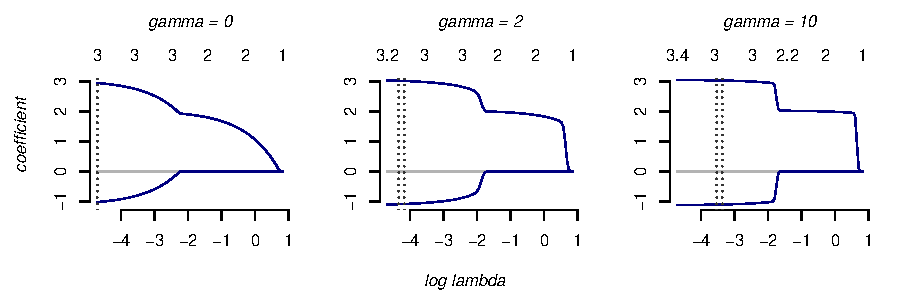
\includegraphics[width=6.5in]{../graphs/gamlr_eg}
\vskip -.25cm
\caption{\label{gamlr_eg} Gamma lasso estimation on $n=10^3$ 
 observations of $y_i = 4 +
3x_{1i} - x_{2i} + \varepsilon_i$, where $\varepsilon_i \stackrel{ind}{\sim} \mr{N}(0,1)$ and
$\{x_{1i},x_{2i},x_{3i}\}$ are marginally standard normal with correlation of
0.9 between covariates ($x_{3i}$ is spurious). The penalty path has $T=100$
segments, $\lambda^1 = n^{-1}\left| \sum_i x_{1i}y_i\right|$, and $\delta =
0.01^{1/99}$. Degrees of freedom are on top and vertical lines mark AIC and
BIC selected models (see Sections \ref{dof}-\ref{selection}).}
\end{figure}



\section{Bayesian motivation}
\label{bayes}

Consider the Bayesian lasso \citep{park_bayesian_2008}, where each $\beta_j$ is
assigned an independent Laplace distribution prior with scale $\tau_j>0$,
\begin{equation}\label{blasso}
\beta_j \sim \mr{La}\left(\tau_j\right) =
\frac{\tau_j}{2}\exp\left[ -\tau_j|\beta_j| ~\right].
\end{equation}
Typically, scale parameters $\tau_1 =
\ldots = \tau_p$ are set as a single shared value, say $n\lambda/\phi$ where
 $\phi$ is the exponential family dispersion (e.g. Gaussian variance
$\sigma^2$ or 1 for the binomial).   Posterior
maximization under the prior in (\ref{blasso}) is then lasso estimation.  In a
fully Bayesian analysis, $\lambda$ is assigned a hyperprior and coefficient
estimates are integrated over its posterior.

Instead of working from shared scale, assume an independent gamma $\mr{Ga}(s,1/\gamma)$
hyperprior with `shape' $s$ and `scale' $\gamma$ for each $\tau_j$, such that
$\ds{E}[\tau_j] = s\gamma$ and $\mr{var}(\tau_j) = s\gamma^2$.  Then the
{\it joint} prior for both coefficient and scale is
\begin{equation}\label{glprior}
\pi(\beta_j,\tau_j) = \mr{La}\left(\beta_j ;~ \tau_j\right)
\mr{Ga}\left(\tau_j;~ s,\gamma^{-1}\right) = \frac{ 1}{2\Gamma({s})} 
\left(\frac{\tau_j}{\gamma}\right)^{s}
               \exp\left[-\tau_j(\gamma^{-1}+|\beta_j|)\right].
\end{equation}
The gamma hyperprior is conjugate here, implying a $\mr{Ga}\left(s+1, ~1/\gamma +
|\beta_j|\right)$ posterior for $\tau_j \mid \beta_j$ with conditional
posterior mode (MAP) at $\hat\tau_j = \gamma s/(1 + \gamma |\beta_j|)$.

Write $s = n\lambda/(\gamma\phi)$, such that
$\ds{E}[\tau_j] = n\lambda/\phi$ and $\mr{var}(\tau_j) =
\gamma\ds{E}[\tau_j]$. Then the MAP scale estimate is $\hat\tau_j =
\omega_j(n\lambda/\phi)$ with $\omega_j = (1+\gamma|\beta_j|)^{-1}$,
and the gamma lasso of Algorithm \ref{gammalasso} appears through a sequence of MAP estimates
 under the joint prior in (\ref{glprior}).  

 \vskip .1cm
At each $\lambda^t$:
 \begin{itemize}
 \item \vskip -.25cm
use the most recent coefficient estimate to fix 
 $\hat\tau^t_j = (n\lambda^t/\phi)/(1+\gamma|\beta^{t-1}_j|)$.
 \item\vskip -.25cm
find $\bs{\hat\beta}^t$ to maximize the posterior under $\mr{La}(\hat\tau^t_j)$
coefficient priors. 
\end{itemize}

\noindent While clearly easier to compute, this sequential `greedy' MAP seems
a poor cousin to an actual joint MAP estimate
-- i.e., that which maximizes the posterior for both $\bs{\tau}$ and
   $\bs{\beta}$. For example, our estimates
   are  sensitive  to  path step-size: as $\delta \rightarrow 1$
    GL approaches the joint MAP, and it gets further from this solution as
   $\delta$ decreases. However, we'll see later that hedging away from joint
   optimality has useful stabilization effects in addition to making for much
   faster analysis. 
   First, we need to look a bit deeper at
   MAP estimation under our Bayesian model.


\subsection{Log penalization}
\label{logpen}

Consider joint MAP estimation of $[\bs{\tau},\bs{\beta}]$ 
   under the prior in (\ref{glprior}), where we've suppressed $\alpha$ for simplicity.
By taking negative logs and removing constants, this is equivalent
to solving
\begin{equation}\label{gljoint}
\min_{\beta_j\in\ds{R},~\tau_j \in \ds{R}^{+}}~~
\phi^{-1}l(\bs{\beta}) + \sum_j \left[\tau_j(\gamma^{-1}+|\beta_j|) - s\log(\tau_j)\right].
\end{equation}
By concentrating-out of $\bs{\tau}$, it is straightforward to show that (\ref{gljoint}) is equivalent 
to the objective 
\begin{equation}\label{logobj}
\min_{\beta_j\in\ds{R},~\tau_j \in \ds{R}^{+}}~~
\phi^{-1}l(\bs{\beta}) + \sum_j  s\log(1+\gamma|\beta_j|)
\end{equation}

\begin{prop}\label{penprop}
  $\bs{\hat\beta}$ solves (\ref{logobj}) if and only if it is also in
  the solution to (\ref{gljoint}).
\end{prop}
\begin{proof}
  The conditional posterior mode for each $\tau_j$ given $\beta_j$
  is $\tau(\beta_j) = \gamma s/(1 + \gamma|\beta_j|)$.  Any joint solution
  $[\bs{\hat\beta},\bs{\hat\tau}]$ for (\ref{gljoint}) thus
  consists of $\hat{\tau}_{j} = \tau(\hat\beta_{j})$;
  otherwise, it is always possible to decrease the objective by
  replacing $\hat\tau_{j}$. Setting each $\tau_j = 
  \tau(\beta_j)$ in (\ref{gljoint}) and removing constant terms yields
  (\ref{logobj}).  Moreover, the solution to (\ref{gljoint}) solves
  (\ref{logobj}): otherwise, there would need to be a point on the
  profile slice of (\ref{gljoint}) defined by $\tau_{j} =
  \tau(\hat\beta_{j})$ that is lower than its minimum.
\end{proof}

Cost function  $c(\beta_j) = s\log(1+\gamma|\beta_j|)$, where $s,\gamma>0$, is referred
to as the log penalty; it is concave with curvature $-s/(\gamma^{-1}+|\beta_j|)^2$ and
spans the range from $L_0$ ($\gamma\rightarrow \infty$) to $L_1$ ($\gamma\rightarrow 0$)
costs.  It appears under a variety of parameterizations and names in the
literature; see \citet{mazumder_sparsenet_2011} and applications in
\citet{friedman_fast_2008}, \citet{candes_enhancing_2008},
\citet{cevher_learning_2009}, \citet{taddy_multinomial_2013} and \citet{armagan_generalized_2013}. 
The penalty is illustrated in Figure \ref{solution}.


\begin{figure}[tbh]
\vskip -.25cm
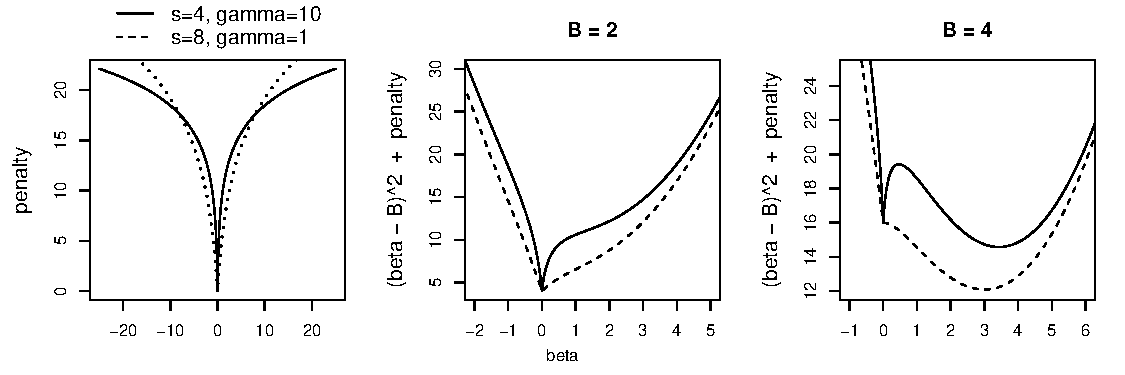
\includegraphics[width=6.4in]{../graphs/solution}
\caption{\label{solution} Log penalties $c(\beta) = s\log(1 + \gamma|\beta|)$ 
and penalized objectives $(\beta-B)^2 + c(\beta)$.}
\end{figure}



\subsection{Generalized double Pareto priors}

For a Bayesian it is odd to be solving for $\bs{\tau}$ rather than
marginalizing over its uncertainty.  However, recognizing the functional form
of a gamma density  in (\ref{glprior}), $\pi(\beta_j,\tau_j)$ integrates over
$\tau_j$ to yield the marginal prior $ \pi(\beta_j) = 0.5s\left( 1+
\gamma|\beta_j|\right)^{-(s+1)}$. This is the generalized double Pareto
density, as in  \citet{armagan_generalized_2013}. Since $-\log \pi(\beta_j)
\propto (s+1)\log(1 + \gamma|\beta_j|)$, the {\it profile} MAP solution to
(\ref{gljoint}), which is also the log penalized estimator from
(\ref{logobj}), gains additional interpretation as the {\it marginal} MAP for
$\bs{\beta}$ under $\mr{Ga}(s-1,1/\gamma)$ hyperpriors on each $\tau_j$.

\section{Implementation via coordinate descent}
\label{implement}

We use Coordinate descent \citep[CD; e.g.,][]{luenberger_linear_2008} to minimize
(\ref{l1pen}) at each step along the path. CD is a local optimization
algorithm that cycles through minimization of the conditional objective for
individual parameters when the remaining parameters are fixed.  It is
conceptually simple, easy to code, and well-suited to optimizations with
hot-start initialization. Algorithms of this type have have become dominant in
$L_1$ penalized estimation since the work by \citet{friedman_pathwise_2007} and
\citet{wu_coordinate_2008}.

Our CD routine, outlined in Algorithm \ref{bmove}, is a solver for penalized
weighted least squares problems as defined in equation (\ref{newton}) below.
This applies directly in Gaussian regression, and for non-Gaussian models  we
follow \citet{friedman_regularization_2010} and apply CD inside an outer loop
of iteratively re-weighted least-squares \citep[IRLS;
e.g.,][]{green_iteratively_1984}. Given current parameter values
$\bs{\hat\beta}$, the Newton-Raphson update for maximum likelihood estimation
is $\bs{\beta} = \bs{\hat\beta} - \bm{H}^{-1}\bm{g}$, where $\bm{H}$ is the
information matrix with elements $h_{jk} = \partial^2 l/\partial
\beta_j\partial \beta_k |_{\bs{\hat\beta}}$ and $\bm{g}$ is coefficient
gradient (see Appendix \ref{models}). For exponential family linear models we
can write $\bm{H} = \bm{X}'\bm{V}\bm{X}$ and $\bm{g} = \bm{X}'\bm{V}(\bm{z} -
\bs{\hat\eta})$, where $\bm{V} = \mr{diag}(\bm{v})$, $\bm{v} = [v_1\ldots
v_n]$ are `weights', $\bm{z} = [z_1\ldots z_n]$ are transformed `response',
and $\hat\eta_i = \hat\alpha + \bm{x}_i\bs{\hat\beta}$.  In Gaussian
regression,  $v_i = 1$, $z_i=\hat\eta_i - y_i$, and the update is an exact
solution. For binomial regression, $v_i = q_i(1-q_i)$ and $z_i = \hat\eta_i -
(y_i-q_i)/v_i$, where $q_i = (1 + \exp[-\hat\eta_i])^{-1}$ is the  estimated
probability of success.

This yields $\bs{\beta} = (\bm{X}'\bm{V}\bm{X})^{-1}\bm{X}'\bm{V}\bm{z}$, such
that the Newton update solves a weighted least-squares problem.   Adding $L_1$
costs,  the minimization objective from (\ref{l1pen}) becomes
\begin{equation} \label{newton}  \argmin_{\alpha,\beta_1 \ldots \beta_p \in
\ds{R}} \sum_i \frac{v_i}{2}(\alpha + \bm{x}_i'\bs{\beta} - z_i)^2  + n\sum_j \omega_j
\lambda |\beta_j|. \end{equation} Our solver iterates between CD on
(\ref{newton}) and,  for non-Gaussian models, updates to $\bm{v}$ and
$\bm{z}$. Each $t^{th}$ segment IRLS routine initializes $[\hat \alpha,
\bs{\hat \beta}]$ at solutions for $\lambda^{t-1}$, or at $[\hat \alpha,
\bm{0}]$ for $t=1$.  In the {\tt gamlr} implementation, a full pass update of
all parameters is done only at the first CD iteration; otherwise coordinates
with currently inactive (zero) $\hat\beta_j$ are not updated. Once the descent
converges for this {\it active set}, IRLS $\bm{v}$ and $\bm{z}$ are updated
and we begin a new CD loop with a full pass update.  The routine stops when
maximum squared change in $\beta_j$ scaled by its information over one of
these full pass updates is less than some tolerance threshold, ${\tt thresh}$.
The default in {\tt gamlr} uses a relative tolerance of $10^{-7}$ times null
model deviance.  \footnote{Under high collinearity one can accelerate convergence via a
quasi-Newton step \citep[e.g.,][]{lange_numerical_2010} as in Appendix
\ref{qn}, but given path hot starts this is usually not
worth the extra computational overhead.}

\vspace{.25cm}
\begin{algorithm}[ht]
\vspace{.25cm}
\caption{Coordinate descent\label{bmove}}

\vskip .15cm
\hskip .5cm Set ${\tt vh_j} = \sum_i v_i(x_{ij} - \bar x_j)^2$ 
and ${\tt vx_j} = \sum_i v_ix_{ij}$ for $j=1\ldots p$.

\vskip .15cm
\hskip .5cm while $\displaystyle \max_{j = 1\ldots p} {\tt vh_j}\Delta_j^2 > {\tt thresh}$:

\vskip .15cm
\hskip 1.5cm for {j=1\ldots p}:


\vskip .15cm
\hskip 2.5cm set ${\tt vg_j} = -\sum_i x_{ij}v_i(z_i-\hat\eta_i)$ and ${\tt ghb} = {\tt vg_j} - {\tt vh_j}\hat\beta_j$


\vskip .25cm
\hskip 2.5cm if $|{\tt ghb}| < n\lambda^t\omega^t_j$:~ $\Delta_j = -\hat\beta_j$

\vskip .1cm
\hskip 2.5cm else:~ $\Delta_j = -({\tt vg_j} - \mr{sign}({\tt ghb}) n\lambda^t\omega^t_j)/{\tt vh_j}$.

\vskip .25cm
\hskip 2.5cm  update $\hat\beta_j \stackrel{+}{=} \Delta_j$,
$\hat\alpha \stackrel{+}{=} -{\tt vx_j}\Delta_j$, 
and $\bs{\hat\eta} = \hat\alpha + \bm{X}'\bs{\hat\beta}$.

\vskip .25cm

\end{algorithm}


\subsection{Descent convergence}

 Despite the non-differentiability of $|\beta_j|$ at zero,
\citet{tseng_convergence_2001} establishes local convergence for CD on
(\ref{newton}) as a consequence of penalty separability: the 
non-differentiable part of our objective is a sum of functions on only a single
coordinate.  Thus CD solves each weighted least squares problem, and  the full
algorithm converges if IRLS does.  For non-Gaussian models this is not always
guaranteed, but divergence is rare and we find the algorithm reliable in
practice.


\subsection{Software}

The algorithm is implemented in {\tt c} as part of the {\tt gamlr} package for
{\sf R}. This software is available with documentation on {\tt
cran.r-project.org} and versioned source code is at {\tt
github.com/mataddy/gamlr}.  Usage of {\tt gamlr} mirrors that of its convex
penalty analogue {\tt glmnet} \citep{friedman_regularization_2010}, the
fantastic and widely used package for costs between $L_1$ and $L_2$
norms. In the lasso case ($\gamma=0$), the two algorithms are essentially
equivalent.



\section{Diminishing bias}
\label{concave}

The defining distinction between the gamma lasso and the standard lasso is
that cost gradient for each $\beta_j$ is decreasing as a function of the size
of its effect  on the likelihood. This occurs algorithmically: if the signal
is strong enough that $\hat \beta^t_j$ is nonzero at $\lambda_t$,  the penalty
at segment $t+1$ is deflated by the factor $1/(1+ \gamma|\beta^t_j|)$ at the
next path segment (see also (\ref{twostep}), the GL two-step thresholding
operator). Consider the log penalty that occurs as $\lambda^t \rightarrow
\lambda^{t-1}$. Under our GL parametrization, the log penalty curvature is
$-n\lambda\gamma/(1+\gamma|\beta_j|)^2$: it is strictly decreasing with
$|\beta_j|$ and goes to zero as $|\beta_j| \rightarrow \infty$. This can be
observed in the left panel of Figure \ref{solution}, and larger $\gamma$
causes the penalty to flatten faster.


We refer to this property of diminishing penalty curvature as `unbiasedness
for large signals'. It is {\it the} reason why one would use concave
penalization instead of $L_1$ or convex alternatives.  Theoretically, it is
the primary necessary condition for a penalized estimator to have
oracle properties: a class of results showing that coefficient
estimates under large $n$ will be the same as if you knew which
should be zero.  \citet{fan_variable_2001} introduce the framework,
\citet{fan_nonconcave_2004} allow $p$ to grow slowly with $n$, 
and \citet{armagan_posterior_2013} provide results specific to log penalization.
Oracle properties make strong assumptions
about near-sparsity of true $\bs{\beta}$, but they form a popular
 approximation framework for evaluating  
high-dimensional estimators. 

There are also a variety of practical reasons for seeking diminishing bias.
First, having large signals estimated without attenuation can increase model
sparsity. This is useful from a purely computational perspective whenever
storage is an issue, say, with distributed massive data analysis
\citep{taddy_distributed_2013}. In causal inference procedures, where
penalized projection from $\bm{x}$ on $y$ is intended to control for
confounding variables rather than for pure prediction,
\citet{belloni_inference_2012} advocate use of unbiased coefficient estimates.
Finally, many
practitioners familiar with classical methods (and versions of subset
selection) will seek out low-bias estimates, regardless of the application.


\subsection{Related estimators}
\label{lla}


Many algorithms have been contributed to accompany the literature on concave
regularization. For example, aforementioned SCAD and MC+ penalties are
implemented for least-squares  in {\tt SIS} and {\tt plus} {\sf R} packages,
respectively.  This software is more prototypical than the industrial
strength tools (like {\tt glmnet}) available for convex regularization.

The recent SparseNet framework of \citet{mazumder_sparsenet_2011} contributes
a  fast class of coordinate descent routines for generic concave penalized
path estimation. The algorithm uses CD to first fit a lasso path and, for each
$\lambda$ on this path, adapts coefficient estimates along a second grid of
increasing concavity specifications (analogous to increasing values of our
$\gamma$). An  implementation for Zhang's MC+ penalty is in the {\tt
sparsenet} package for {\sf R}, and it is the best available software we've
found.  Indeed, we find very similar runtimes for {\tt sparsenet} and roughly
equivalent loops of {\tt gamlr} over multiple $\gamma$; neither is
consistently faster across problems.  The advantage of {\tt gamlr} is that
each different $\gamma$ specification can be run in parallel (and you only
need use one $\gamma$ if you wish), whereas the {\tt sparsenet}
algorithm moves through a grid of both $\lambda$ and $\gamma$ in order to
avoid minor modes in the nonconvex penalized objective.


The SparseNet authors argue that it is important in CD  to solve exactly the
coordinate-wise objective at each update.  This will make the solution less
sensitive (but not insensitive) to initial values.  Thus if the bimodal
objective in the right-most panel of Figure \ref{solution} represents a
coordinate update, one should make sure to find the major mode out near
$\beta=4$. For log penalization, \cite{taddy_multinomial_2013} finds these
exact solutions by solving a simple quadratic equation.  Unfortunately, even
this simple exact method becomes prohibitively expensive for $p$ and $n$ above
a few thousand (unless, like in SparseNet, you 
derive good hot-starts from a joint $[\gamma,\lambda]$ grid).   The gamma lasso only ever attempts to solve convex
optimization problems along the path, so convergence to minor modes is a non-issue.

 It turns out that the GL algorithm is quite closely related to the `local
linear approximation' (LLA) routines that are criticized as sub-optimal in
\cite{mazumder_sparsenet_2011}.  Of course, when the objective itself is
uncertain (and needs to be chosen via model selection) the properties of the
entire path (e.g. stability) are more important than a single point being
optimal under a fixed specification.  Indeed,  a new literature
\citep{loh_regularized_2013,wang_optimal_2013}  holds that, under limited
penalty concavity, all local solutions  should be within {\it statistical}
precision of the global solution.  These papers are technically difficult and
the ideas are early in development, but they support the simple point that one
should not worry too much about global solutions under a fixed penalty when
the optimal specification of that penalty is itself unknown.

\subsection{Local linear approximation and one-step estimators}

A local linear approximation replaces the concave cost function $c$ in a
penalized deviance with its tangent at the current estimate,
$c'(\hat\beta)\beta$.  The approximate objective is then  a standard lasso
(solvable by, say, the CD of Section \ref{implement}), and one iterates
between updating $c'(\hat\beta)$ and solving the implied $L_1$ penalized
minimization problem. \citet{candes_enhancing_2008} apply LLA to the log
penalty, in which case $c'(\beta) = s \gamma / (1 + \gamma |\beta|)$.  The
method  is simple and locally convergent, but  it is especially sensitive to
initial starting location.  Consider approximating the log penalized
objectives of Figure \ref{solution} with LLA $l(\beta) + c'(0)|\beta|$:  the
approximation will minimize at $\beta=0$  until $|l'(\beta)| > c'(0)$, even
when the true objective $\beta\neq 0 $ local minimum is much lower. Thus in a
path estimation algorithm, LLA sticks at zero until it jumps all the way out
to near the MLE.

Despite this issue, \citet{zou_one-step_2008} present numerical and
theoretical evidence that simple LLA does well in practice. For us, the
relevant contribution of Zou and Li is their one-step implementation of LLA
and its analysis: each GL path segment executes a version of this one-step LLA
algorithm. One-step estimation is a general technique
\citep[e.g.,][]{bickel_one-step_1975} which amounts to taking as your estimator
the first step of an iterative approximation to some objective function.   In
general, one-step estimators are usually accompanied by results claiming that
they can be `as good' asymptotically as the full-step solution {\it if} the
initial estimates are `good enough'.  Since the efficiency of regularization
paths depends upon segment solutions being good starts for the next segment,
they form a natural setting for such techniques.

In the context of LLA for the log penalty, one-step estimation implies solving
$\bs{\hat\beta}$ to minimize deviance under  penalties $\lambda|\beta_j|/(1 +
\gamma \hat\beta_j^0)$, where $\bs{\hat\beta}^0$ are some initial estimates of
the coefficients.  For Zou and Li, $\bs{\beta}^0$ is set to the
MLE (or left unspecified), whereas in  the gamma lasso we set it to the
previous path segment's estimate. The theoretical framework of one-step
estimation, and results from  Zou and Li in particular, apply
directly to our GL estimator (note that the adaptive lasso of
\citet{zou_adaptive_2006} can also be cast as a one-step LLA). This includes
oracle properties if the regularization parameter is appropriately chosen. The
Zou and Li result on continuity is  more general than our
simple statement in Section \ref{stability}:  one-step LLA is continuous if
and only if $c'(\beta)$ is continuous for $|\beta|>0$.  

\section{Comparison to $L_0$ penalized optimization}

In the following two subsections we provide results for weighted $L_1$ estimation in two areas commonly motivating use of diminishing-bias-type penalties: prediction using a sparse basis, and support recovery.  We compare to optimal $L_0$ penalized estimation here, even though in the later section on stability it is clear that $L_0$ penalized estimation may not be the best choice even if it were feasible.


\subsection{Sparse Approximation for Prediction}

One advantage of diminishing bias is that you can reduce the difference between estimated $\hat y$ and prediction from an optimal sparse approximation to
$\bs{\beta}$ (e.g., the MLE restriced to large coefficients).  For any support subset $S \subset 1\ldots p$ with cardinality $|S|=s$ and complement $S^c = \{1\ldots p\}\setminus S$, denote vectors
restricted to $S$ as $\bm{\beta}_S = [\beta_j:j\in S]'$, matrices as $\bm{X}_S$, etc.  Use superscripted $\bs{\beta}^S$ to denote the coefficient vector for OLS restricted to $S$: that is, $\bs{\beta}^S_S = (\bm{X}_S'\bm{X}_S)^{-1}\bm{X}_S'\bm{y}$ and $\beta^{S}_j = 0~\forall~j\notin S$.  Moreover, 
$\bm{e}^S = \bm{y}-\bm{X}\bs{\beta}^\nu = (\bm{I}-\bm{H}^S)\bm{y}$ and 
$\bm{H}^S = \bm{X}_S(\bm{X}_S'\bm{X}_S)^{-1}\bm{X}_S'$ are the residuals and hat (projection) matrix respectively from OLS restricted to $S$.

We'll use the following simple result for stagewise regression -- iterative fitting of new covariates to the residuals of an existing linear model (as in, e.g., \citealt{goldberger_stepwise_1961}). It bounds the reduction in variance due to a new stagewise-estimated coefficient.
\begin{lemma}\label{SSElemma}
Say $\mr{MSE}_S = \|\bm{X}\bs{\beta}^S-\bm{y}\|^2/n$ and 
$\mr{cov}(\bs{x}_j,\bm{e}^S) = \bs{x}_j'(\bm{y}-\bm{X}\bs{\beta}^S)/n$ are sample variance and covariances.  Then for any $j \in 1\ldots p$, 
\[
\mr{cov}^2(\bs{x}_j,\bm{e}^S) \leq \mr{MSE}_S - \mr{MSE}_{S\cup j}
\]
\end{lemma}
\begin{proof}
From the well-known property on the correlation coefficient ($R^2$) for linear models,   
in-sample correlation and variances are such that
\[
\frac{\mr{cov}^2(\bs{x}_j,\bm{e}^S)}{\mr{var}(\bs{x}_j)\mr{var}(\bm{e}^S)} = 1 - \frac{\mr{var}(\bm{e}^S-\tilde\beta_j\bs{x}_j)}{\mr{var}(\bm{e}^S)}
\]
where $\tilde\beta_j = \bs{x}_j'\bm{e}^S/(\bs{x}_j'\bs{x}_j)$ is the stagewise coefficient estimate.  Since $\mr{var}(\bs{x}_j)=1$, multiplying everything by $\mr{var}(\bm{e}^S)$ yields $\mr{cov}^2(\bs{x}_j,\bm{e}^S) =
\mr{var}(\bm{e}^S) - \mr{var}(\bm{e}^S-\tilde\beta_j\bs{x}_j)
\leq \mr{var}(\bm{e}^S) - \mr{var}(\bm{e}^{S\cup j})$.
The last inequality holds because $\bm{e}^{S\cup j}$, residuals from OLS on $\bm{X}_{S\cup j}$, have the smallest-possible sum of squares for that set of covariates.  With $\mr{var}(\bm{e}^S) = \mr{MSE}_S$, etc, we are done.
\end{proof}

In addition, we need to define {\it restricted eigenvalues} (RE) on the observed gram matrix.  
\begin{definition}\label{redef}
The restricted eigenvalue is
$
\phi^2(L,S) = \min_{\{\bm{v}: \bm{v}\neq \bm{0},~|\bm{v}_{S^c}| \leq L\sqrt{s}\|\bm{v}_S\|\}}\frac{\|\bm{X}\bm{v}\|^2}{n\|\bm{v}\|^2}$.
\end{definition}
\noindent The specific RE in Definition (\ref{redef}) matches the `adaptive restricted eigenvalues' of \cite{buhlmann_statistics_2011}.  These and related RE quantities are common in prediction and estimation results for both $L_1$ and concave penalization schemes.  See the remarks for more detail.

Finally, our result derives a bound on the distance between prediction rules based on $L_0$ and weighted $L_1$ penalized estimation.
\begin{theorem} \label{sparseapprox}  Consider squared-error loss $l(\bs{\beta}) =
\frac{1}{2}\|\bm{X}\bs{\beta}-\bm{y}\|^2$, and suppose $\bs{\beta}^{\nu}$ minimizes the $L_0$ penalized objective $l(\bs{\beta}) + n\nu\sum_{j=1}^p\ds{1}_{\{\beta_j\neq0\}}$ with $\bs{\beta}^\nu = \bs{\beta}^S$ and $|S|=s<n$.   
Write $\bs{\hat\beta}$ as solution to the weighted $L_1$ minimization $l(\bs{\beta}) + n\lambda\bs{\omega}'|\bs{\beta}|$. 

Then  
$\omega^{\mr{min}}_{S^c}\lambda > \sqrt{2\nu}$ while $\phi^2(L,S) > 0$ implies
\begin{equation} \label{sparseineq}
\frac{\|\bm{X}(\bs{\hat\beta}-\bs{\beta}^\nu)\|^2}{n}\leq
\frac{4\lambda^2 \|\bs{\omega}_S\|^2}{\phi^2(L, S)}
\end{equation} 
with the restricted eigenvalue defined for 
 $L = \frac{\|\bs{\omega}_S\|}{\sqrt{s}}(\omega^{\mr{min}}_{S^c}-\sqrt{2\nu}/\lambda)^{-1}$.
\end{theorem}

\begin{proof}
From the definitions of $\bs{\hat\beta}$ and $\bs{\beta}^\nu = \bs{\beta}^S$, 
\begin{align}\label{predconv}
\frac{1}{2}\|\bm{X}\bs{\hat \beta}-\bm{y}\|^2 + n\lambda\bs{\omega}'|\bs{\hat\beta}| & ~~=~~ \frac{1}{2}\|\bm{X}(\bs{\hat\beta}-\bs{\beta}^\nu)\|^2 + \frac{1}{2}\|\bm{e}^S\|^2 - \bm{\hat y}'\bm{e}^S+ n\lambda\bs{\omega}'|\bs{\hat\beta}|\\
& ~~~~~~~~~\leq~~ \frac{1}{2}\|\bm{X}\bs{\beta}^\nu-\bm{y}\|^2 + n\lambda\bs{\omega}'|\bs{\beta}^\nu| ~~=~~ \frac{1}{2}\|\bm{e}^S\|^2 + n\lambda\bs{\omega}_S'|\bs{\beta}^\nu_S|\notag
\end{align}
  Since $\bm{\hat y}'\bm{e}^S = \bm{\hat y}'(\bm{I}-\bm{H}^S)\bm{y} =
\bs{\hat\beta}'\bm{X}'(\bm{y}-\bm{X}\bs{\beta}^\nu) = 
\sum_{j\in S^c} \hat\beta_j\bs{x}_j'(\bm{y}-\bm{X}\bs{\beta}^\nu)
$,
 we can apply Lemma \ref{SSElemma} followed by $\bs{\beta}^\nu$ being optimal under $L_0$ penalty $\nu$ to get 
\begin{equation} \label{L0ineq}
\left(\frac{\bs{x}_j'(\bm{y}-\bm{X}\bs{\beta}^\nu)}{n}\right)^2
\leq \mr{MSE}_S - \mr{MSE}_{S\cup j} < 2\nu ~~~\forall~j
\end{equation}
so that $|\bm{\hat y}'\bm{e}^S| = |\bs{\hat\beta}_{S^c}\bm{X}_{S^c}'(\bm{y}-\bm{X}\bs{\beta}^\nu)| < n\sqrt{2\nu}|\bs{\hat\beta}_{S^c}|$.

Applying (\ref{L0ineq}) inside (\ref{predconv}),
\begin{align}\label{predconvineq}
\frac{1}{2}\|\bm{X}(\bs{\hat\beta}-\bs{\beta}^\nu)\|^2
  + n\left(\omega^{\mr{min}}_{S^c}\lambda-\sqrt{2\nu}\right)|\bs{\hat\beta}_{S^c}|
  &~\leq~ n\lambda\bs{\omega}_{S}'|\bs{\hat\beta}_{S}-\bs{\beta}^\nu_S|
  ~\leq~ n\lambda\|\bs{\omega}_S\|\|\bs{\hat\beta}_{S}-\bs{\beta}^\nu_S\|.
\end{align}
Given $\omega^{\mr{min}}_{S^c}\lambda > \sqrt{2\nu}$,
difference $\bs{\hat\beta}-\bs{\beta}^\nu$ is in the RE support for 
$L=\frac{\|\bs{\omega}_S\|}{\sqrt{s}}(\omega^{\mr{min}}_{S^c}-\sqrt{2\nu}/\lambda)^{-1}$ and thus $\|\bs{\hat\beta}_{S}-\bs{\beta}^\nu_S\| \leq \|\bm{X}(\bs{\hat\beta}-\bs{\beta}^\nu)/\sqrt{n}\|/\phi(L,S)$.  Finally, applying this inside (\ref{predconvineq}) yields
\begin{align}
\frac{1}{2}\|\bm{X}(\bs{\hat\beta}-\bs{\beta}^\nu)\|^2
  &~\leq~ \frac{\sqrt{n}\lambda\|\bs{\omega}_S\|\|\bm{X}(\bs{\hat\beta}-\bs{\beta}^\nu)\|}
  {\phi(L, S)}.
\end{align}
Dividing each side by $\sqrt{n}\|\bm{X}(\bs{\hat\beta}-\bs{\beta}^\nu)\|/2$ and squaring gives the result.
\end{proof}

\noindent {\bf Remarks}

\vskip .25cm
\noindent $\bullet$~~   The comparison to $L_0$ estimation, as opposed to some assumed model truth, is key to the simplicity of our inequality in (\ref{sparseineq}).  The result is finite sample exact, and completely non-parametric -- it makes no reference to the true distribution of $\bm{y}\mid \bm{X}$.  Indeed, if we are to make such assumptions, Theorem \ref{sparseapprox} provides bounds on the distance between a weighted lasso and optimal sparse prediction.  The next remark is an example.

\vskip .25cm
\noindent $\bullet$~~ From \cite{efron_estimation_2004}, the $C_p$ statistic
\citep{mallows_comments_1973} implies that choosing $S$ to minimize
$\mr{MSE}_S + 2s\sigma^2/n$, Mallows' unbiased estimate of residual variance,
is optimal for minimizing prediction error on $\bm{y} \sim
(\bm{f},\sigma^2\bm{I})$ -- that is, for $y_i$ independent with means $f_i$
and shared variance $\sigma^2$. Theorem (\ref{sparseapprox}) with $\nu = \sigma^2/n$ and $L = \frac{\|\bs{\omega}_S\|}{\sqrt{s}}\left(\omega^{\mr{min}}_{S^c}- \sqrt{2}\sigma/(\lambda\sqrt{n})\right)^{-1}$ provides a comparison between weighted $L_1$ estimation and $C_p$-optimal prediction.\footnote{We work with
$C_p$ here, rather than $AIC$ or $AICc$, since $C_p$ is conveniently defined
the scale of squared errors.} Note that, since the condition on minimum $S^c$ weights has become
$\omega^{\mr{min}}_{S^c} > (\sigma/\lambda)\sqrt{2/n}$, comparison to $C_p$ suggests we can use larger $\gamma$ (faster diminishing bias) with large $n$ or small $\sigma$.


\vskip .25cm
\noindent $\bullet$~~  Plausibility of the restricted eigenvale assumption $\phi(L,S) > 0$ depends critically upon $L$.  Here, the assumption is less restrictive if we can reduce $\|\bs{\omega}_S\|$ without making $\omega^{\mr{min}}_{S_c}$ small.  For example, the next sub-section suggests using large $\gamma$ so long as $\lambda$ is big enough to avoid false discovery. More generally, \cite{raskutti_restricted_2010} show that similar conditions hold  with very high probability for $\bm{X}$ drawn from a broad class of Gaussian distributions.  \cite{bickel_simultaneous_2009} provide a nice overview of sufficient conditions, and \cite{buhlmann_statistics_2011} have extensive discussion and examples related to restricted eigenvalue assumptions.


\subsection{False Discovery Control}

Two related goals in high-dimensional estimation are  support recovery -- having the set $\{j: \hat\beta_j \neq 0\} = \{j: \beta_j \neq 0\}$ for some `true' $\bs{\beta}$ -- and  sign recovery -- in addition, $\mr{sgn}(\bs{\hat\beta}) = \mr{sgn}(\bs{\beta})$.  For standard lasso estimated $\bs{\hat\beta}$, many authors have shown \citep[e.g.,][]{buhlmann_statistics_2011,zou_adaptive_2006} that to get exact support recovery asymptotically or with high probability requires an {\it irrepresentability condition} which limits the size of least-squares projections from `true support' onto spurious covariates.  
\begin{definition} 
The $(\theta,S,\bm{v})$-irrepresentable condition for $\theta\in[0,1]$ and $\bm{v}\in \ds{R}^s$ holds that, 
\begin{equation}\label{irrep}
|\bs{x}_j'\bm{X}_S(\bm{X}_S'\bm{X}_S)^{-1}\bm{v}| \leq \theta ~~\forall~j\notin S
\end{equation}
\end{definition}

A common form of (\ref{irrep}) has $\bm{v}=\bm{1}$.\footnote{\cite{wainwright_sharp_2009} shows that the irrepresentable condition with $\theta=1$ and $\bm{v}=\bm{1}$ is necessary for lasso sign recovery in the {\it noiseless} estimation setting.} In this case, it
is a strict design restriction; for example,
\citet{buhlmann_statistics_2011} have a single variable that is
highly correlated with many columns of $\bm{X}_S$ leading to failure. Much
of the literature on concave penalized estimation has focused on achieving
support recovery {\it without} such conditions; see, e.g.,
\cite{fan_strong_2014} for a recent overview that provides finite sample
theory.  

Our exposition here will compare $\hat S = \{j: \hat\beta_j \neq 0\}$, for $\bs{\hat\beta}$ from weighted $L_1$ penalized estimation, to $S = \{j: \beta^\nu_j \neq 0\}$ for $\beta^\nu$ from $L_0$ penalized estimation as in Theorem \ref{sparseapprox}.  The result uses an irrepresentable condition with $\bm{v} = \bs{\omega}_S$, an assumption that becomes less restrictive as one is able to shrink weights $\omega_j$ for $j\in S$.

A path-wise interpretation of Theorem \ref{signrecov} is that the gamma lasso achieves exact sign recovery if $(i)$ holds until $(ii)$ occurs.  We can re-state the result in terms of false positives relative to $\bs{\beta}^{\nu}$ along the path, with $\bs{\hat\beta}^t$ and $\hat S_t = \{j: \hat\beta^t_j\neq 0\}$ the  weighted lasso coefficient estimates and support under $\bs{\omega}^t$ and $\lambda_t$ at path segment $t$.
\begin{corollary}
Under the setting of Theorem \ref{signrecov}, if $\hat S_{t-1} \cap S^c = \varnothing$ and $\lambda_t > \sqrt{2\nu}$ then
\begin{equation}\label{falsepos}
\|\bm{X}_{S^c}'\bm{X}_S(\bm{X}_S'\bm{X}_S)^{-1}\bs{\omega}^t_S\|_{\infty} \leq 1 - \frac{\sqrt{2\nu}}{\lambda_t} ~~\Rightarrow~~\hat S_{t} \cap S^c = \varnothing.
\end{equation}
\end{corollary}
\noindent 
The results uses $\hat S_{t-1} \cap S^c = \varnothing \Rightarrow \omega_{S^c}^{t~\mr{min}} = 1$ for the GL algorithm.  So long as $\lambda_t$ is large enough, (\ref{falsepos}) suggests that  big $\gamma$ (for fast diminishing $\omega_j$) will help control false discovery.  Of course, the momment $\hat S_{t-1} \cap S^c \neq \varnothing$,  a large $\gamma$ allows spurious covariates to enter with very little shrinkage and can move the fit arbitratily far away from $L_0$-optimal support.

\vskip .25cm
\noindent {\bf Remarks}
\vskip .25cm
\noindent $\bullet$~~ From Theorem 7.4 in \cite{buhlmann_statistics_2011}, 
the irrepresentability condition holds with 
$|\bs{x}_j'\bm{X}_S(\bm{X}_S'\bm{X}_S)^{-1}\bs{\omega}_S|
\leq \frac{\|\bs{\omega}_S\|}{\sqrt{s}}\theta_{\mr{adap}}(S)$ where $\theta_{\mr{adap}}(S)$ is their `adaptive restricted regression' coefficient.  Of direct interest here, they show that $\theta_{\mr{adap}}(S) \leq \sqrt{s}/\Lambda_{\mr{min}}(S)$ where $\Lambda_{\mr{min}}(S) = \mr{min}_{\{\bm{v}:\|\bm{v}\|=1\}}\bm{v}'\left(\frac{\bm{X}_S'\bm{X}_S}{n}\right)\bm{v}$ is the minimum eigenvalue of $\bm{X}_S'\bm{X}_S/n$.  Thus, $(i)$ can be replaced by the restriction $\Lambda_{\mr{min}}(S) \geq \|\bs{\omega}_S\|(1 - \sqrt{2\nu}/(\omega_{S^c}^{\mr{min}}\lambda))^{-1} = \sqrt{s}L$, with $L$ from Theorem \ref{sparseapprox}. Small values for $L$ are key in both predictive performance and support recovery.

\vskip .25cm
\noindent $\bullet$~~ Without any irrepresentability condition,  limits on false discovery are more pessimistic.  For example, under the setting of Theorem \ref{sparseapprox},  local optimality
conditions imply that for $j \in S^c \cap \hat S$ we have
$n\lambda \omega_j = |\bs{x}_j'(\bm{X}\bs{\hat\beta}-\bm{y})| \leq
|\bs{x}_j'\bm{X}(\bs{\hat\beta}-\bs{\beta}^\nu)| + |\bs{x}_j'\bm{e}^S| \leq
n\left(2\|\bs{\omega}_S\|/\phi(L,S) + \sqrt{2\nu}/\lambda\right) ~\forall~j$. 
Dividing by $n\lambda\omega_j$ and counting yields
\begin{equation}\label{pessimism}
|S^c \cap \hat S| \leq \left|\frac{1}{\bs{\omega}_{S^c \cap \hat S}}\right|
\left(\frac{2\|\omega_S\|}{\phi(L,S)} + \frac{\sqrt{2\nu}}{\lambda}\right)
\end{equation}
Thus, without the ability to
make $\omega_j$ very big for $j \in S^c$ (e.g., as in a thresholding procedure
like that of \citealt{zhou_thresholding_2009}), the result in (\ref{pessimism}) has little to say about false discovery control.
See 
\cite{buhlmann_statistics_2011} for more detail on related ideas.


\section{Stability and Continuity}
\label{stability}


The benefits of Section \ref{concave} come at a price: if the penalty is
concave, the negative log posterior is not necessarily convex.  This can
be seen in the right two panels of Figure \ref{solution}: the objectives are
concave approaching the origin, and can even become bi-modal.

The obvious effect of a non-convexity is computational:  the models take
longer to fit. The genius of LARS and the lasso is that entire regularization
paths are easy to calculate {\it because}  estimates change slowly along those
paths.  In contrast, the previous segment $\bs{\hat\beta}^{t-1}$ will not be a
good hot-start for $\bs{\hat\beta}^{t}$ if the solution paths have
discontinuity jumps. This causes a corresponding jump in computation time; for
example, Figure \ref{nhltime} shows timings growing rapidly after
 this threshold (around $1<\gamma<10$) for the hockey data  of Section \ref{nhl}.
Here the cost difference is mere seconds, but in larger $n$ and $p$
applications the jumps become prohibitively expensive.

\begin{figure}[bht]
\vskip -.5cm
\centering
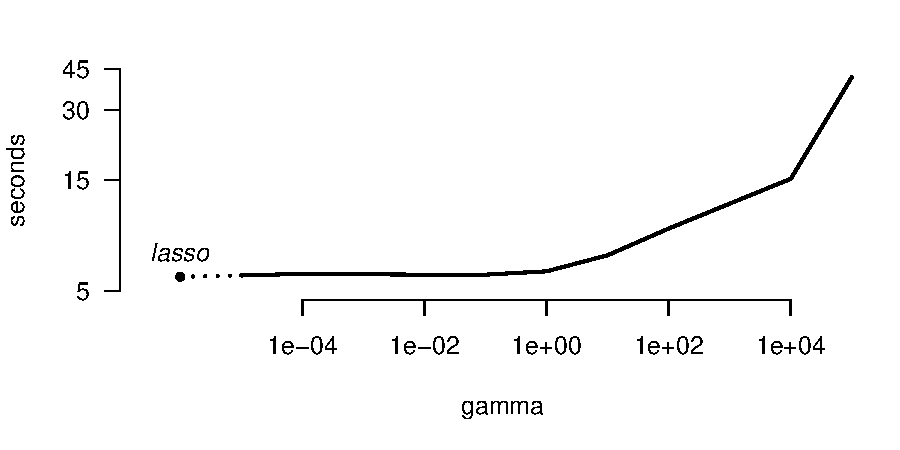
\includegraphics[width=5.5in]{../graphs/nhl_time}
\vskip -.25cm
\caption{\label{nhltime} 
Timings for the hockey data fits of Section \ref{nhl}
on a length-100 grid with $\lambda^{100} = 0.01\lambda^1$. This
used a high absolute convergence tolerance of $10^{-10}$; results are less dramatic under default settings.}
\end{figure}

Such discontinuities occur if the objective is concave at the origin.
Consider the solid line in the right panel of Figure \ref{solution}: under
small permutation to penalty $\gamma s$, the solution moves between $0$ and
near $4$. When conditional updates in coordinate descent (see Section
\ref{implement}) have this shape, all other dimensions of the model fit need to
change dramatically depending upon such thresholds.   Moreover, finding a {\it
global} solution is computationally intractable if the objective is
non-convex; this issue is discussed in  detail in Section
\ref{lla}.


A more subtle possible consequence of concavity is estimator instability. Path
discontinuities will cause jumps in the implicit estimation function for
$\bs{\hat\beta}$, such that small data jitter leads to large changes in model
fit. As every statistics student should know, mean squared error for $\hat y$
as a predictor of $y$ can be written as the sum of squared bias
$(y-\ds{E}[\hat y])^2$ plus estimator variance $\mr{var}(\hat y)$.  Thus
instability leads to lower quality prediction due to a large increase in the
sampling variance. As detailed in the classic \cite{breiman_heuristics_1996}
discussion, the effects of instability are especially dramatic when doing
model selection, since variability of this choice explodes with the estimation
variance for each individual candidate model (see also Section
\ref{selection}).

Given these issues, the benefits of concave penalties (i.e., the diminishing bias
of Section \ref{concave}) are only worthwhile so long as we are able to
remain stable.  The rest of this section looks first at what this means in
terms of our Bayesian model and second at how sub-optimality of the gamma
lasso as a joint MAP actually stabilizes the procedure.

\subsection{Prior variance}

For orthogonal inputs, the penalized objective becomes concave only if
negative log likelihood coordinate curvature $h_j = \partial^2 l(\bs{\beta})/\partial
\beta_j^2$, which does not depend upon $y$ for exponential families, is less
than the absolute value of the curvature on the cost function for $\beta_j$.
Absolute curvature for the log penalty is $s\gamma^2$ at the origin, and less
elsewhere, such that  the objective in (\ref{logobj}) is guaranteed convex if
$s\gamma^2 < h_j$.  For correlated inputs, one has objective convexity if the
minimum eigenvalue of $\bm{H}$, the Hessian matrix of second derivatives of
$l(\bs{\beta})$, is greater than $s\gamma^2$.\footnote{ \noindent If $\nu$ is an
eigenvalue of $\bm{H}$, then $(\bm{H} -
\nu \bm{I})\bm{v} = 0$ for some nonzero $\bm{v}$; the negative log posterior
Hessian at zero is $\bm{H} - s\gamma^2\bm{I}$ and $(\bm{H} - s\gamma^2\bm{I} + s\gamma^2\bm{I} -
\nu \bm{I})\bm{v} = 0$ so that 
$\nu - s\gamma^2$ is an eigenvalue of the minimization objective.}

Recognizing $\gamma^2 s$ as the variance of a $\mr{Ga}(s,\gamma^{-1})$
distribution, the above can be given a clear Bayesian interpretation in the
context of our model from Section \ref{bayes}:  the joint MAP is stable
(changes little under small data jitter)  if the prior variance on each
$\tau_j$ coefficient scale is less than the minimum eigenvalue of the likelihood information
matrix $\bm{H}$. For Gaussian regression with standardized orthogonal
covariates, $h_j = \sum_i x_{ij}^2 = n$ and we get a simple rule: the joint
MAP is stable  if prior variance on each $\tau_j$  is
less than the number of observations.  For logistic regression you need
$\mr{var}(\tau_j) < n/4$ to get the same guarantee. And for marginal rather
than joint MAP estimation you need $\mr{var}(\tau_j) + \gamma^2$ less than $n$
or $n/4$.


\subsection{Stability of the gamma lasso}

A rigorous definition of stability can be expressed in terms of the continuity
of  estimators as a function of $\bm{y}$, the observed response.  In
particular, Lipschitz continuity of such functions is of primary importance in
estimation; e.g., for unbiased risk assessment as in
\cite{stein_estimation_1981}.  Many popular concave cost functions, such as
the SCAD penalty of \cite{fan_variable_2001} and the MC+ penalty of
\citet{zhang_nearly_2010}, have been engineered to be Lipschitz continuous (at
least under certain parameterizations).  It turns out that gamma lasso
estimators have this property.

Say $f(b)$ is the implicit function for $\hat\beta$ as a function of the MLE
$b$.  $f$ is said to be Lipschitz continuous if  $ |f(b_1)-f(b_2)| \leq
L|b_1-b_2| $ for some finite constant $L$ on all $b_1,b_2$ in the domain of
$f$. If the MLE $b$ is itself Lipschitz with respect to $\bm{y}$, then we'll
say that the estimator is Lipschitz stable.    Consider the single-coefficient
two step path $[\hat\beta^0,\hat\beta^1]$ on $[\lambda,\delta\lambda]$ for
$0<\delta<1$, such that $\hat\beta^0$ is the lasso estimate under $\tau =
\lambda$ and $\hat\beta^1$ is the lasso estimate under $\tau =
\delta\lambda/(1+\gamma|\hat\beta^0|)$. Given MLE $b$ we can re-write
$\hat\beta^1$ as \begin{equation}\label{twostep} f(b) = \left(b -
\frac{\delta\lambda}{1+\gamma(b-\lambda)_+}\right)_+  \end{equation} where
$\gamma,\lambda,\delta >0$, $\lambda < \infty$, $\delta<1$.  We call this the
gamma-lasso thresholding operator.

\begin{prop} For $\gamma<\infty$ the GL thresholding  operator in
(\ref{twostep}) is Lipschitz continuous. \end{prop} \begin{proof} Take two
arbitrary MLE $b_1 > b_2 >0$;  other configurations work similarly.   If
$f(b_1) = f(b_2) =0$ the condition holds trivially.   If $f(b_1) > f(b_2) >
0$, then  $|f(b_1) - f(b_2)| = b_1 - b_2 + \delta\lambda (A_1 -
A_2)/[(1+A_1)(1+A_2)] \leq (1+\delta\lambda \gamma)|b_1-b_2|$, where $A_k =
\gamma(b_k-\lambda)_{+}$. Finally, if $f(b_1)>0, f(b_2)=0$ then w.l.o.g.~write $b_1 = \delta\lambda + \epsilon$, $b_2 = \delta\lambda$, for $\epsilon  = |b_1-b_2| > 0$, so
that 
\begin{equation}\label{lipeq}
 |f(b_1) - f(b_2)| =\epsilon  
 + \delta\lambda\left(1 - \frac{1}
 {1 + \gamma(\delta\lambda + \epsilon - \lambda)_+}\right).
 \end{equation} 
For $\epsilon \leq (1-\delta)\lambda$, (\ref{lipeq}) becomes $ \epsilon$.  Otherwise (\ref{lipeq}) is 
less than $\epsilon + \delta\lambda
\left(\gamma\epsilon/(1+\gamma\epsilon)\right) < (1+\delta\gamma\lambda)\epsilon$.
\end{proof}

Note the connection between path continuity and estimator stability: if there
are jumps in a solution path as a function of $\lambda$, then Lipschitz
continuity is impossible. To see this, note that one could choose $b_1$ and
$b_2$ arbitrarily close but on either side of the discontinuity threshold
$\lambda$.  For this reason it is clear that Lipschitz continuity {\it does not
hold} for $\gamma =\infty$.

\subsection{Forward vs Backward Selection}

Most authors looking at weighted $L_1$ estimation start from more complex models to derive the penalty weights -- in our context, use $\bs{\beta}^0$ for $\lambda_0$ to define weights at $\lambda_1 \geq \lambda_0$.  This approach seems to have developed because, with the exception of marginal regression-based weights, it easier to derive oracle inequalities for this `backwards' rather than our `forwards' algorithm.  A quick result here argues that, in any case, the greedy forward algorithm provides lower variance prediction than a backwards algorithm.
\begin{prop}
forward var $<$ backward var
\end{prop}
We're not certain that, e.g., support recovery has lower probability under the forward rather than backward algorithm.  However, we don't doubt this to be the case, and it would be another example of the stability vs selection trade-off.

\section{Degrees of freedom}
\label{dof}

An estimation algorithm's degrees of freedom ($df$) is a key property in
determining its tendency to over or under fit.  We use it in Section
\ref{selection} as the  basis for selecting the optimal model along a
fitted regularization path, so it is a key ingredient for practical
application of the GL algorithm.  

In an unpenalized linear model, the degrees of freedom is just the number of
estimated parameters.  More generally, it can be defined as
\citep[e.g.][]{efron_least_2004} $df = \sigma^{-2} \sum_i \mr{cov}(\hat y_i,
y_i)$ where $\hat y_i$ is the estimated prediction rule for observation $y_i$
and $\sigma^2$ is residual variance. Given an estimator that is Lipschitz
continuous with respect to $\bm{y}$, as demonstrated in Section
\ref{stability} \citep[or in ][]{zou_one-step_2008} for our GL path segments,
the SURE framework of \cite{stein_estimation_1981} applies and we get a more
workable version of this definition,  $df = \ds{E}\left[\sum_i \partial \hat
y_i/\partial y_i\right]$.

Consider the case of a single coefficient $\beta$ estimated via least-squares
under $L_1$ penalization $\tau$.   Write gradient at zero $g = -\sum_i
x_iy_i$ and curvature $h = \sum_i x_i^2$ and set $\varsigma = -{\tt sign}(g)$.
Then the prediction rule for $y$ given $x$ is $\hat y =
x(\varsigma/h)(|g|-\tau)_+$ with  derivative $\partial \hat y/\partial y =
x_i^2/h \ds{1}_{[|g|<\tau]}$, yielding  the SURE degrees of freedom expression
$df = \ds{E}\left[ \ds{1}_{[|g|<\tau]} \right]$.   For many orthogonal
covariates, we get $\hat y = \sum_j x_j(\varsigma_j/h_j)(|g_j|-\tau_j)_+$ and
the degrees of freedom becomes  
\begin{equation} \label{sure} df = \sum_j
\ds{E}\left[ \ds{1}_{[|g_j|<\tau_j]} \right].
\end{equation}
\cite{zou_degrees_2007} plug sample gradients into (\ref{sure}) to derive
$\hat p = \sum_j |g_j| < \tau_j = \sum |\hat\beta_j| \neq 0$, the number of
nonzero  coefficients, as an unbiased estimator of model
degrees of freedom.


We'll use the same tactic of plugging-in observed gradient.  However, for the
GL algorithm each $\tau_j$ is a function of $y$.  Moreover, unlike $g_j$, our
observed $\hat\tau_j$ have been optimized to fit the data and thus  plugging
them into (\ref{sure}) would yield a biased (low) estimate of $df$. Fortunately,
interpreting the GL algorithm as an estimator for the Bayesian  hierarchical
model of Section \ref{bayes},  we do have a guess for each $\tau_j$ that is
independent from the data: our $\mr{Ga}(s,1/\gamma)$ hyperprior. This implies the
{\it gamma lasso estimator for degrees of freedom} \begin{equation}
\label{edf} df^t = \sum_j \mr{Ga}(|g_{j}|;~ n\lambda^t/(\gamma\phi),
1/\gamma). \end{equation}  The number of unpenalized coefficients (e.g.,~1 for
$\alpha$) is always added to this to get total $df$.  For Gaussian regression,
where $\phi$ is unknown, we just use the fitted mean square error $\hat\phi^t
= \sum_i (y_i - \hat y_i)^2/n$. Under (\ref{edf}) as $\gamma \rightarrow 0$,
$df^t \rightarrow \hat p$, the lasso $df$ of Zou et al. As $\gamma \rightarrow
\infty$, $df^t$ becomes $p$ and we assign full model $df$ for all steps of the
GL subset selection algorithm.


In the non-orthogonal case, $g_{j} = g_j(0)$ becomes a function of all of the
elements of $\bs{\beta}$.     One option would be to plug-in the null model
gradients (i.e. for all zero coefficients), but with any multicollinearity
this yields too-large $df$ values (e.g., almost immediately $df \approx p$ in
our simulations of Section \ref{sim}). Instead we use the most recent $g_j$ at
which $\hat\beta^t_j=0$, such that the effect of previously in-the-model
variables has been remove from our plug-in gradient.  This appears to work
well in practice, requires no extra computation (since we already need these
values in CD), and has the advantage of maintaining $df = \hat p$ for $\gamma
= 0$.

\section{Selection}
\label{selection}

Penalized estimation does not perform model selection. Rather, its value is as
a technique to quickly enumerate,  along regularization paths, a set of
plausible candidate models.   In the simplest setting, the models are  indexed
by a single penalty size parameter, say $\lambda$. This acts as a {\it
squelch}: it suppresses noise to focus on the true input signal.  The model
selection problem is then to choose $\lambda$ so that models estimated under
that  squelch are neither over nor under fit.

\subsection{Cross validation}

The simplest metric of a model's quality is how well it predicts for data {\it
that you have not observed} drawn from the same (assumed independent across
observations) generating process as the sample $\mc{S} = [\bm{X},\bm{y}]$.  We
measure this in terms of deviance under the assumed likelihood: $-2$ times the
fitted log likelihood minus the log likelihood for a saturated model (with
$p=n$ free parameters).  Since evaluation on actually unobserved data is
impossible, it is common to use $K$-fold cross-validation \cite[CV; see][for
an overview]{efron_estimation_2004} to estimate  predictive performance: split
the sample into $K$  evenly-sized disjoint subsets (folds) $\mc{S}_k$,  and
$K$ times fit a regularization path given $\mc{S} \setminus \mc{S}_k$.
Predictions for data in the left-out fold are  used to calculate `out-of-
sample' (OOS) deviance   along each regularization path. Given CV results, one
selects $\lambda$ according to some criterion and re-fits the model on the
entire dataset under this penalty.  The usual rules are either
$\lambda_{\mr{min}}$, the penalty with minimum average OOS error, or
$\lambda_{1\mr{se}}$, the largest penalty with average OOS error no more than
1 standard error away from that at $\lambda_{\mr{min}}$ (to account for
downward bias in deviance at $\lambda_{\mr{min}}$ as an estimator of true
prediction deviance).

CV is super useful, and some form of it features in most applied problems, but
it does have some serious weaknesses. As a basic point, $K$ should be bigger
than 2-3 (5-10 is typical); if a single path-fit is expensive then doing it
$K$ times will be impractical.  More subtly, in contemporary Big data problems
the data is distributed: it is too large to store on a single machine.
Analysts can use conditional independence factorization to work in parallel on
data subsets \citep[e.g.,][]{taddy_distributed_2013}, but a computational
bottleneck results if you need to communicate across such subsets for OOS
experimentation.  Thus there are settings where we'll need to replace CV with
performance estimates that can be derived from  a single model fit.


\subsection{Information Criteria}

An alternative approach to measuring predictive performance follows \citet[see
also \citealt{efron_estimation_2004}]{mallows_comments_1973} in estimating
true OOS error via the `Information Criterion', \begin{equation}\label{cp}
\text{IC}(k) = 2l(\hat\alpha,\bs{\hat\beta}) + k\times df \end{equation} where
$k$ is a complexity penalty.  We are able plug-in the $df^t$ degrees of
freedom heuristic from (\ref{edf}) here, and the IC-selected model is that
which minimizes the criterion in (\ref{cp}).

The two most common information criteria specifications are the AIC's $k=2$
\citep[derived from information theoretic arguments
in][]{akaike_information_1973} or the BIC's $k=\log(n)$ \citep[derived from
approximation to marginal likelihood for a Bayesian model
in][]{schwarz_estimating_1978}.  Our experience is that the BIC-selected model
works better  for OOS prediction in big-$p$/small-$n$ applications, but it does tend to yield very simple models and the
AIC will be preferred if you need to tell a story about weak signals or if $n\gg p$ 
(e.g., as in Section \ref{nhl}).  See \citet{flynn_efficiency_2013} for discussion of the AIC and its adaptation for selection in high-dimensional penalized regression.


Note that with both IC and CV it is best to use `stable'
models. For IC, Section \ref{dof} outlines how the required $df$ can be
approximated easily only for models that are Lipschitz continuous.  And
\citet{breiman_heuristics_1996} argues that CV does a poor job of evaluating
unstable models: it evaluates  {\it average} performance of given $\lambda$
as a squelch, but this is a good guess at the
performance of a single particular fit (which is what we actually have)  only
if models estimated at this $\lambda$ are not too variable across samples --
that is, if the model is stable.  Thus a simple argument for stability is as
follows: regularization paths enumerate candidate models that we must choose
amongst, and we have good tools for such choice only if the paths are
continuous.

\subsection{Laplace approximation to the marginal likelihood}

An alternative  interpretation for information criteria is as Laplace
approximation \citep{de_bruijn_asymptotic_1958} to the negative log of the
{\it marginal likelihood} $\mr{p}(\bm{y} | \lambda) = \int_{\bs{\theta}}
\mr{p}( \bm{y} | \bs{\theta} ) d\mr{P}_\lambda(\bs{\theta})$, where
$\bs{\theta}$ is the set of model parameters and
$\mr{P}_\lambda(\bs{\theta})$ is its prior distribution parametrized by
 $\lambda$. For this interpretation of the BIC to apply
informally here, $\bs{\theta}$ is a 
parametrization of $\bm{X}\bs{\beta}$ in the subspace that results after constraining $\sum_j |\beta_j|$  and $\mr{P}_\lambda(\bs{\theta})$ is the
{\it unit information} Gaussian prior centered at  MLE $\bs{\hat\theta}$ with
variance $-\partial^2\log\mr{p}(\bm{y}| \bs{\theta} )/\partial\theta_j^2
|_{\bs{\hat\theta}}$. See \citet{kass_bayes_1995} and
\citet{spiegelhalter_bayesian_2002} for discussion and references on the
connection between Bayes and IC.



A more direct approach to Bayesian model selection would just approximate the
marginal likelihood for one of models in Section \ref{bayes}:
$\int_{\bs{\beta}} \mr{p}( \bm{y} | \bs{\beta} ) d\mr{P}_\lambda(\bs{\beta})$.
Unfortunately, Laplace approximation to this integral -- replacing the
integrand with a normal centered at  $\bs{\hat\beta}$ --  is inappropriate if
the posterior is not differentiable at some $\hat\beta_j=0$.
\citet{zhou_path_2012} propose  `empirical Bayes factors' (EBF) that
approximate instead $\int_{\bs{\beta}_\mc{A}} \mr{p}( \bm{y} |
\bs{\beta}_\mc{A} ) d\mr{P}_\lambda(\bs{\beta}_\mc{A})$, the marginal
likelihood over only active-set $\bs{\beta}_\mc{A} = \{\beta_j: \hat\beta_j
\neq 0\}$.\footnote{\citet{yuan_efficient_2005} take a similar approach under
a different prior on shared Laplace scale $\tau$, and derive this active set
integral as an upper bound on true marginal likelihood.} However we find in
simulation that this technique, which is much more computationally intensive,
does worse than simple BIC using plug-in $df^t$.

\section{Simulation}
\label{sim}

\begin{table}[p]\vspace{-.5cm}
\caption[l]{\it Predictive Mean Square Error\hfill}
\vspace{-.5cm}
\small\setstretch{1}
\begin{center}
\begin{tabular}{l*{5}{c}|r}
 & lasso & GL $\gamma=2$ & GL $\gamma=10$ & marginal AL & sparsenet MC+  &  \\
\cline{1-7}
CV.1se & 4.4 & 4.3 & 4.8 & 4.3 & 4.2 &\\
CV.min & 4.1 & {\bf 4} & 4.3 & 4.1 & {\bf 4} &  $\mr{sd}(\bm{\mu})/\sigma=2$ \\
AICc & 4.3 & 4.1 & 4.1 & 4.2 & & $\rho=0$ \\
AIC & 5 & 5.2 & 5.2 & 4.1 & & \multirow{2}{*}{$C_p$ mse = 3.5} \\
BIC & 5.6 & 5.1 & 5.7 & 4.9 & & \\
 \hline 
CV.1se & 3.1 & 3 & 3.4 & 3.1 & 2.9 &\\
CV.min & 2.9 & {\bf 2.8} & 3 & 3 & {\bf 2.8} &  $\mr{sd}(\bm{\mu})/\sigma=2$ \\
AICc & 3 & {\bf 2.8} & 2.9 & 3 & & $\rho=0.5$ \\
AIC & 3.4 & 3.5 & 3.5 & 2.9 & & \multirow{2}{*}{$C_p$ mse = 2.4} \\
BIC & 4.4 & 3.7 & 4.1 & 3.8 & & \\
 \hline 
CV.1se & 2.4 & 2.4 & 2.6 & 2.6 & 2.3 &\\
CV.min & 2.3 & {\bf 2.2} & 2.3 & 2.4 & {\bf 2.2} &  $\mr{sd}(\bm{\mu})/\sigma=2$ \\
AICc & 2.4 & {\bf 2.2} & 2.3 & 2.5 & & $\rho=0.9$ \\
AIC & 2.6 & 2.7 & 2.7 & 2.4 & & \multirow{2}{*}{$C_p$ mse = 1.9} \\
BIC & 3.5 & 3 & 3.3 & 3.2 & & \\
 \hline 
CV.1se & 17 & 16.9 & 18 & 15.6 & 16.4 &\\
CV.min & 15.6 & 15.6 & 16.5 & 15.7 & 15.6 &  $\mr{sd}(\bm{\mu})/\sigma=1$ \\
AICc & 15.8 & {\bf 15.5} & 15.9 & 15.6 & & $\rho=0$ \\
AIC & 21.3 & 22.2 & 22.2 & 17 & & \multirow{2}{*}{$C_p$ mse = 13.8} \\
BIC & 20.8 & 19.2 & 23.4 & 17.7 & & \\
 \hline 
CV.1se & 12 & 11.7 & 12.7 & 11.1 & 11.3 &\\
CV.min & 10.9 & 10.8 & 11.5 & 11 & 10.8 &  $\mr{sd}(\bm{\mu})/\sigma=1$ \\
AICc & 11.1 & {\bf 10.7} & 10.8 & 11 & & $\rho=0.5$ \\
AIC & 14.4 & 14.9 & 14.9 & 11.8 & & \multirow{2}{*}{$C_p$ mse = 9.2} \\
BIC & 15.8 & 14.4 & 16.1 & 13.4 & & \\
 \hline 
CV.1se & 9.4 & 9.2 & 10.1 & 9.1 & 8.9 &\\
CV.min & 8.6 & {\bf 8.5} & 9 & 8.8 & {\bf 8.5} &  $\mr{sd}(\bm{\mu})/\sigma=1$ \\
AICc & 8.8 & {\bf 8.5} & {\bf 8.5} & 8.8 & & $\rho=0.9$ \\
AIC & 11.2 & 11.6 & 11.6 & 9.1 & & \multirow{2}{*}{$C_p$ mse = 7.3} \\
BIC & 12.7 & 12.1 & 12.9 & 11.4 & & \\
 \hline 
CV.1se & 60.9 & 61.2 & 61.3 & 57.8 & 61 &\\
CV.min & 57.8 & 59.8 & 60.6 & 60.5 & 57.9 &  $\mr{sd}(\bm{\mu})/\sigma=0.5$ \\
AICc & {\bf 57.6} & 60 & 61.4 & 59 & & $\rho=0$ \\
AIC & 88.4 & 92.5 & 92.5 & 73.2 & & \multirow{2}{*}{$C_p$ mse = 53.5} \\
BIC & 61.3 & 61.3 & 61.3 & 60.6 & & \\
 \hline 
CV.1se & 41.1 & 41.2 & 41.2 & 39.8 & 41.2 &\\
CV.min & 39.9 & 40.7 & 41 & 41.3 & 39.9 &  $\mr{sd}(\bm{\mu})/\sigma=0.5$ \\
AICc & {\bf 39.6} & 40.5 & 41.3 & 40.5 & & $\rho=0.5$ \\
AIC & 59.4 & 61.9 & 61.9 & 49.9 & & \multirow{2}{*}{$C_p$ mse = 35.9} \\
BIC & 41.2 & 41.2 & 41.2 & 41 & & \\
 \hline 
CV.1se & 32.6 & 32.6 & 32.6 & 31.8 & 32.6 &\\
CV.min & 31.8 & 32.3 & 32.5 & 32.4 & 31.8 &  $\mr{sd}(\bm{\mu})/\sigma=0.5$ \\
AICc & {\bf 31.5} & 32.1 & 32.6 & 32.2 & & $\rho=0.9$ \\
AIC & 46.4 & 48.6 & 48.6 & 38.1 & & \multirow{2}{*}{$C_p$ mse = 28.3} \\
BIC & 32.6 & 32.6 & 32.6 & 32.5 & & \\
 \hline \end{tabular}
\end{center}
\vspace{-1cm}
\end{table}

\begin{table}[p]\vspace{-.5cm}
\caption[l]{\it Predictive $R^2$\hfill}
\vspace{-.5cm}
\small\setstretch{1}
\begin{center}
\begin{tabular}{l*{5}{c}|r}
 & lasso & GL $\gamma=2$ & GL $\gamma=10$ & marginal AL & sparsenet MC+  &  \\
\cline{1-7}
CV.1se & 0.71 & 0.72 & 0.68 & 0.72 & 0.73 &\\
CV.min & 0.73 & {\bf 0.74} & 0.72 & 0.73 & {\bf 0.74} &  $\mr{sd}(\bm{\mu})/\sigma=2$ \\
AICc & 0.72 & 0.73 & 0.73 & 0.73 & & $\rho=0$ \\
AIC & 0.67 & 0.66 & 0.66 & 0.73 & & \multirow{2}{*}{$C_p ~ R^2$ = 0.77} \\
BIC & 0.63 & 0.67 & 0.63 & 0.68 & & \\
 \hline 
CV.1se & 0.7 & 0.71 & 0.67 & 0.7 & 0.72 &\\
CV.min & 0.72 & {\bf 0.73} & 0.7 & 0.71 & {\bf 0.73} &  $\mr{sd}(\bm{\mu})/\sigma=2$ \\
AICc & 0.71 & {\bf 0.73} & 0.72 & 0.71 & & $\rho=0.5$ \\
AIC & 0.67 & 0.66 & 0.66 & 0.71 & & \multirow{2}{*}{$C_p ~ R^2$ = 0.77} \\
BIC & 0.57 & 0.64 & 0.6 & 0.63 & & \\
 \hline 
CV.1se & 0.7 & 0.71 & 0.68 & 0.68 & 0.72 &\\
CV.min & 0.72 & {\bf 0.73} & 0.71 & 0.7 & {\bf 0.73} &  $\mr{sd}(\bm{\mu})/\sigma=2$ \\
AICc & 0.71 & {\bf 0.73} & 0.72 & 0.7 & & $\rho=0.9$ \\
AIC & 0.68 & 0.67 & 0.67 & 0.7 & & \multirow{2}{*}{$C_p ~ R^2$ = 0.77} \\
BIC & 0.57 & 0.63 & 0.6 & 0.61 & & \\
 \hline 
CV.1se & 0.31 & 0.31 & 0.27 & 0.36 & 0.33 &\\
CV.min & 0.36 & 0.36 & 0.33 & 0.36 & 0.36 &  $\mr{sd}(\bm{\mu})/\sigma=1$ \\
AICc & 0.35 & {\bf 0.37} & 0.35 & 0.36 & & $\rho=0$ \\
AIC & 0.13 & 0.09 & 0.09 & 0.3 & & \multirow{2}{*}{$C_p ~ R^2$ = 0.44} \\
BIC & 0.15 & 0.22 & 0.04 & 0.28 & & \\
 \hline 
CV.1se & 0.27 & 0.29 & 0.23 & 0.33 & 0.32 &\\
CV.min & 0.34 & {\bf 0.35} & 0.3 & 0.33 & {\bf 0.35} &  $\mr{sd}(\bm{\mu})/\sigma=1$ \\
AICc & 0.32 & {\bf 0.35} & {\bf 0.35} & 0.33 & & $\rho=0.5$ \\
AIC & 0.12 & 0.1 & 0.1 & 0.28 & & \multirow{2}{*}{$C_p ~ R^2$ = 0.44} \\
BIC & 0.04 & 0.13 & 0.02 & 0.19 & & \\
 \hline 
CV.1se & 0.28 & 0.29 & 0.23 & 0.3 & 0.31 &\\
CV.min & 0.34 & {\bf 0.35} & 0.31 & 0.32 & {\bf 0.35} &  $\mr{sd}(\bm{\mu})/\sigma=1$ \\
AICc & 0.33 & {\bf 0.35} & {\bf 0.35} & 0.32 & & $\rho=0.9$ \\
AIC & 0.14 & 0.11 & 0.11 & 0.3 & & \multirow{2}{*}{$C_p ~ R^2$ = 0.44} \\
BIC & 0.03 & 0.07 & 0.01 & 0.13 & & \\
 \hline 
CV.1se & 0.01 & 0 & 0 & {\bf 0.06} & 0 &\\
CV.min & {\bf 0.06} & 0.02 & 0.01 & 0.01 & 0.05 &  $\mr{sd}(\bm{\mu})/\sigma=0.5$ \\
AICc & {\bf 0.06} & 0.02 & 0 & 0.04 & & $\rho=0$ \\
AIC & -0.44 & -0.51 & -0.51 & -0.2 & & \multirow{2}{*}{$C_p ~ R^2$ = 0.13} \\
BIC & 0 & 0 & 0 & 0.01 & & \\
 \hline 
CV.1se & 0 & 0 & 0 & 0.03 & 0 &\\
CV.min & 0.03 & 0.01 & 0 & -0.01 & 0.03 &  $\mr{sd}(\bm{\mu})/\sigma=0.5$ \\
AICc & {\bf 0.04} & 0.01 & 0 & 0.01 & & $\rho=0.5$ \\
AIC & -0.45 & -0.51 & -0.51 & -0.21 & & \multirow{2}{*}{$C_p ~ R^2$ = 0.13} \\
BIC & 0 & 0 & 0 & 0 & & \\
 \hline 
CV.1se & 0 & 0 & 0 & 0.02 & 0 &\\
CV.min & 0.02 & 0.01 & 0 & 0 & 0.02 &  $\mr{sd}(\bm{\mu})/\sigma=0.5$ \\
AICc & {\bf 0.03} & 0.01 & 0 & 0.01 & & $\rho=0.9$ \\
AIC & -0.43 & -0.5 & -0.5 & -0.17 & & \multirow{2}{*}{$C_p ~ R^2$ = 0.13} \\
BIC & 0 & 0 & 0 & 0 & & \\
 \hline 
\end{tabular}
\end{center}
\vspace{-1cm}
\end{table}

\begin{table}[p]\vspace{-.5cm}
\caption[l]{\it False Discovery Rate $\mid$ Sensitivity, relative to $C_p$ model\hfill}
\vspace{-.5cm}
\small\setstretch{1}
\begin{center}
\begin{tabular}{l*{5}{c}|r}
 & lasso & GL $\gamma=2$ & GL $\gamma=10$ & marginal AL & sparsenet MC+  & \\
 \cline{1-7}
CV.1se & 0.49 $\mid$ 0.76 & 0.26 $\mid$ 0.67 & 0.07 $\mid$ 0.56 & 0.43 $\mid$ 0.67 & 0.15 $\mid$ 0.61 &\\
CV.min & 0.65 $\mid$ 0.84 & 0.48 $\mid$ 0.77 & 0.20 $\mid$ 0.65 & 0.57 $\mid$ 0.74 & 0.40 $\mid$ 0.74 &  $\mr{sd}(\bm{\mu})/\sigma=2$ \\
AICc & 0.55 $\mid$ 0.79 & 0.44 $\mid$ 0.76 & 0.37 $\mid$ 0.73 & 0.53 $\mid$ 0.71 & & $\rho=0$ \\
AIC & 0.84 $\mid$ 0.94 & 0.84 $\mid$ 0.93 & 0.84 $\mid$ 0.91 & 0.63 $\mid$ 0.77 & & \multirow{2}{*}{$\bar{s}_{C_p}$ = 123.7} \\
BIC & 0.22 $\mid$ 0.59 & 0.07 $\mid$ 0.53 & 0.02 $\mid$ 0.45 & 0.22 $\mid$ 0.54 & & \\
 \hline 
CV.1se & 0.58 $\mid$ 0.75 & 0.37 $\mid$ 0.67 & 0.12 $\mid$ 0.55 & 0.53 $\mid$ 0.64 & 0.14 $\mid$ 0.58 &\\
CV.min & 0.69 $\mid$ 0.84 & 0.56 $\mid$ 0.77 & 0.27 $\mid$ 0.65 & 0.63 $\mid$ 0.71 & 0.34 $\mid$ 0.69 &  $\mr{sd}(\bm{\mu})/\sigma=2$ \\
AICc & 0.60 $\mid$ 0.77 & 0.50 $\mid$ 0.74 & 0.41 $\mid$ 0.73 & 0.59 $\mid$ 0.69 & & $\rho=0.5$ \\
AIC & 0.84 $\mid$ 0.94 & 0.84 $\mid$ 0.94 & 0.84 $\mid$ 0.92 & 0.67 $\mid$ 0.75 & & \multirow{2}{*}{$\bar{s}_{C_p}$ = 123.5} \\
BIC & 0.29 $\mid$ 0.53 & 0.13 $\mid$ 0.49 & 0.04 $\mid$ 0.44 & 0.31 $\mid$ 0.49 & & \\
 \hline 
CV.1se & 0.59 $\mid$ 0.76 & 0.43 $\mid$ 0.67 & 0.21 $\mid$ 0.56 & 0.54 $\mid$ 0.61 & 0.20 $\mid$ 0.57 &\\
CV.min & 0.69 $\mid$ 0.84 & 0.57 $\mid$ 0.77 & 0.35 $\mid$ 0.66 & 0.63 $\mid$ 0.69 & 0.41 $\mid$ 0.69 &  $\mr{sd}(\bm{\mu})/\sigma=2$ \\
AICc & 0.61 $\mid$ 0.77 & 0.52 $\mid$ 0.74 & 0.43 $\mid$ 0.71 & 0.60 $\mid$ 0.66 & & $\rho=0.9$ \\
AIC & 0.84 $\mid$ 0.94 & 0.84 $\mid$ 0.93 & 0.83 $\mid$ 0.91 & 0.65 $\mid$ 0.71 & & \multirow{2}{*}{$\bar{s}_{C_p}$ = 123.9} \\
BIC & 0.35 $\mid$ 0.51 & 0.20 $\mid$ 0.47 & 0.09 $\mid$ 0.43 & 0.39 $\mid$ 0.47 & & \\
 \hline 
CV.1se & 0.43 $\mid$ 0.58 & 0.18 $\mid$ 0.44 & 0.07 $\mid$ 0.33 & 0.52 $\mid$ 0.62 & 0.26 $\mid$ 0.50 &\\
CV.min & 0.66 $\mid$ 0.73 & 0.43 $\mid$ 0.60 & 0.19 $\mid$ 0.45 & 0.68 $\mid$ 0.73 & 0.57 $\mid$ 0.69 &  $\mr{sd}(\bm{\mu})/\sigma=1$ \\
AICc & 0.60 $\mid$ 0.69 & 0.50 $\mid$ 0.65 & 0.50 $\mid$ 0.63 & 0.62 $\mid$ 0.69 & & $\rho=0$ \\
AIC & 0.90 $\mid$ 0.93 & 0.90 $\mid$ 0.92 & 0.90 $\mid$ 0.89 & 0.79 $\mid$ 0.82 & & \multirow{2}{*}{$\bar{s}_{C_p}$ = 90.0} \\
BIC & 0.07 $\mid$ 0.25 & 0.04 $\mid$ 0.25 & 0.00 $\mid$ 0.04 & 0.17 $\mid$ 0.38 & & \\
 \hline 
CV.1se & 0.52 $\mid$ 0.54 & 0.30 $\mid$ 0.43 & 0.12 $\mid$ 0.32 & 0.61 $\mid$ 0.58 & 0.23 $\mid$ 0.42 &\\
CV.min & 0.70 $\mid$ 0.71 & 0.53 $\mid$ 0.60 & 0.27 $\mid$ 0.45 & 0.71 $\mid$ 0.69 & 0.47 $\mid$ 0.58 &  $\mr{sd}(\bm{\mu})/\sigma=1$ \\
AICc & 0.65 $\mid$ 0.66 & 0.56 $\mid$ 0.63 & 0.56 $\mid$ 0.65 & 0.67 $\mid$ 0.65 & & $\rho=0.5$ \\
AIC & 0.90 $\mid$ 0.94 & 0.90 $\mid$ 0.93 & 0.90 $\mid$ 0.91 & 0.81 $\mid$ 0.81 & & \multirow{2}{*}{$\bar{s}_{C_p}$ = 90.0} \\
BIC & 0.03 $\mid$ 0.07 & 0.05 $\mid$ 0.15 & 0.00 $\mid$ 0.03 & 0.21 $\mid$ 0.26 & & \\
 \hline 
CV.1se & 0.57 $\mid$ 0.54 & 0.40 $\mid$ 0.43 & 0.23 $\mid$ 0.30 & 0.62 $\mid$ 0.53 & 0.32 $\mid$ 0.40 &\\
CV.min & 0.71 $\mid$ 0.72 & 0.57 $\mid$ 0.60 & 0.38 $\mid$ 0.45 & 0.70 $\mid$ 0.65 & 0.55 $\mid$ 0.58 &  $\mr{sd}(\bm{\mu})/\sigma=1$ \\
AICc & 0.66 $\mid$ 0.66 & 0.58 $\mid$ 0.61 & 0.58 $\mid$ 0.62 & 0.69 $\mid$ 0.62 & & $\rho=0.9$ \\
AIC & 0.90 $\mid$ 0.94 & 0.90 $\mid$ 0.92 & 0.90 $\mid$ 0.90 & 0.80 $\mid$ 0.77 & & \multirow{2}{*}{$\bar{s}_{C_p}$ = 89.7} \\
BIC & 0.03 $\mid$ 0.04 & 0.05 $\mid$ 0.08 & 0.00 $\mid$ 0.01 & 0.21 $\mid$ 0.17 & & \\
 \hline 
CV.1se & 0.07 $\mid$ 0.05 & 0.01 $\mid$ 0.01 & 0.01 $\mid$ 0.01 & 0.65 $\mid$ 0.45 & 0.07 $\mid$ 0.04 &\\
CV.min & 0.61 $\mid$ 0.41 & 0.20 $\mid$ 0.13 & 0.07 $\mid$ 0.05 & 0.80 $\mid$ 0.63 & 0.59 $\mid$ 0.40 &  $\mr{sd}(\bm{\mu})/\sigma=0.5$ \\
AICc & 0.64 $\mid$ 0.43 & 0.49 $\mid$ 0.34 & 0.02 $\mid$ 0.01 & 0.76 $\mid$ 0.57 & & $\rho=0$ \\
AIC & 0.94 $\mid$ 0.92 & 0.94 $\mid$ 0.90 & 0.94 $\mid$ 0.90 & 0.90 $\mid$ 0.81 & & \multirow{2}{*}{$\bar{s}_{C_p}$ = 56.5} \\
BIC & 0.00 $\mid$ 0.01 & 0.00 $\mid$ 0.00 & 0.00 $\mid$ 0.00 & 0.07 $\mid$ 0.05 & & \\
 \hline 
CV.1se & 0.04 $\mid$ 0.01 & 0.01 $\mid$ 0.00 & 0.00 $\mid$ 0.00 & 0.70 $\mid$ 0.35 & 0.09 $\mid$ 0.01 &\\
CV.min & 0.56 $\mid$ 0.25 & 0.20 $\mid$ 0.07 & 0.08 $\mid$ 0.03 & 0.82 $\mid$ 0.56 & 0.54 $\mid$ 0.24 &  $\mr{sd}(\bm{\mu})/\sigma=0.5$ \\
AICc & 0.65 $\mid$ 0.31 & 0.43 $\mid$ 0.26 & 0.05 $\mid$ 0.03 & 0.79 $\mid$ 0.49 & & $\rho=0.5$ \\
AIC & 0.94 $\mid$ 0.93 & 0.94 $\mid$ 0.91 & 0.94 $\mid$ 0.91 & 0.91 $\mid$ 0.80 & & \multirow{2}{*}{$\bar{s}_{C_p}$ = 56.3} \\
BIC & 0.01 $\mid$ 0.00 & 0.00 $\mid$ 0.00 & 0.00 $\mid$ 0.00 & 0.06 $\mid$ 0.02 & & \\
 \hline 
CV.1se & 0.03 $\mid$ 0.01 & 0.01 $\mid$ 0.00 & 0.00 $\mid$ 0.00 & 0.68 $\mid$ 0.25 & 0.14 $\mid$ 0.01 &\\
CV.min & 0.53 $\mid$ 0.19 & 0.23 $\mid$ 0.05 & 0.08 $\mid$ 0.02 & 0.82 $\mid$ 0.49 & 0.52 $\mid$ 0.17 &  $\mr{sd}(\bm{\mu})/\sigma=0.5$ \\
AICc & 0.67 $\mid$ 0.27 & 0.41 $\mid$ 0.21 & 0.04 $\mid$ 0.03 & 0.80 $\mid$ 0.44 & & $\rho=0.9$ \\
AIC & 0.94 $\mid$ 0.93 & 0.94 $\mid$ 0.90 & 0.94 $\mid$ 0.90 & 0.90 $\mid$ 0.76 & & \multirow{2}{*}{$\bar{s}_{C_p}$ = 55.8} \\
BIC & 0.01 $\mid$ 0.00 & 0.00 $\mid$ 0.00 & 0.00 $\mid$ 0.00 & 0.08 $\mid$ 0.01 & & \\
 \hline 
 \end{tabular}
\end{center}
\vspace{-1cm}
\end{table}

On an Intel Xeon E5-2670 processor, average time for 5-fold CV with $\mr{sd}(\bm{\mu})/\sigma=1$ and $\phi=1/2$ was around 2 seconds for lasso and marginal regression AL, 3 and 4 seconds for GL with $\gamma=2$ and $\gamma=10$ respectively, and 15-20 seconds for Sparsenet. Sparsenet computation is comparable to a set of {\tt gamlr} runs over a grid of 9 $\gamma$ values.  However, as a path following algorithm and unlike {\tt gamlr}, sparsenet cannot run in parallel over the $\gamma$ grid.   For comparison,  a single run of SCAD on this configuration, using the {\tt ncvreg} R package, took 10 minutes -- clearly limiting the technology to a much smaller set of  applications.\footnote{In a small study, we found that the CV.min selected SCAD performs quite well in prediction --  similarly to the best CV.min methods for each data configuration -- with relatively high values for both false discovery and sensitivity. }

Marginal regression coefficient estimates are often \citep[e.g.,][]{huang_adaptive_2008} suggested as weights for an adaptive lasso in the $p>n$ setting.  Indeed, since marginal correlations tend to have a lower sampling variance than conditional coefficients, this strategy should yield lower variance weights and stable estimation when compared to more complicated weighting schemes.  Our simulation study investigates marginal-correlation-based adaptive lasso.

Our first example uses data simulated independently from the following
$p$-covariate regression.
\begin{align}
\label{simdgp}
\bm{x} &\sim \mr{N}\left(\bm{0},\bs{\Sigma}\right),~~\Sigma_{jk} = 0.9^{|j-k|},~~z_{j} \stackrel{ind}{\sim} \mr{Bin}(0.5)~~\text{for}~~j=1\ldots p,
 \\
y &= \mr{N}(\mu,\sigma^2)~~\text{where}~~\mu = (\bm{x}*\bm{z})'\bs{\beta},~~\beta_j = \frac{1}{j}\exp\left(-\frac{j}{10}\right),~~\text{and}
~~\sigma=1.25\mr{sd}(\mu).\notag
\end{align}
Here, $\mr{sd}(\mu)$ is the sample standard deviation over simulated $\mu_1\ldots\mu_n$.  The true process in (\ref{simdgp}) is not sparse; the $\beta_j$ are actually diminishing in absolute size very slowly.  However $\bm{x}$ is highly
correlated across dimensions and it is useless to estimate the coefficients
for large $j$.  

\begin{figure}[p]
\vspace{-.25cm}
{ \hskip 2.5cm$\bs{\gamma=0}$\hskip 4cm$\bs{\gamma=2}$\hskip 4cm$\bs{\gamma=10}$}

\vskip .2cm
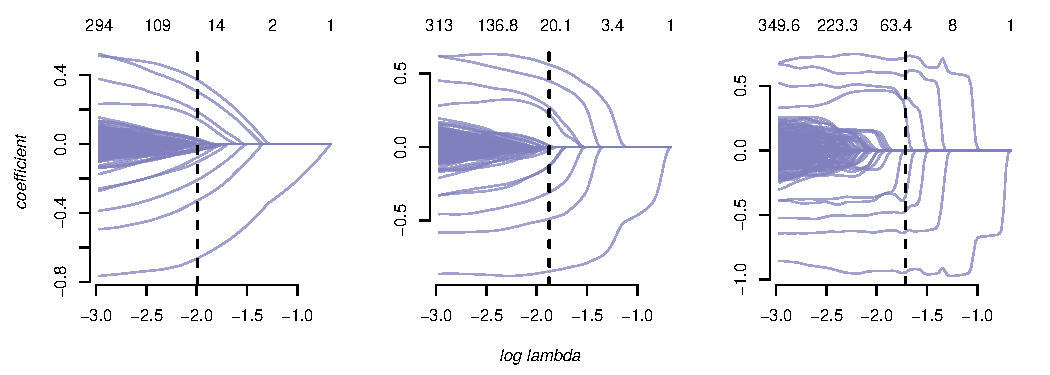
\includegraphics[width=6.5in]{../graphs/sim_paths}
\caption{\label{simpaths} Regularization paths for a single run of our simulated linear regression example, on $\gamma = 0,2,10$ from left.
Vertical lines mark the BIC selection, and  degrees of freedom $df^t$ are along the top. }

\vskip .7cm
{ \hskip 2.5cm$\bs{\gamma=0}$\hskip 4cm$\bs{\gamma=2}$\hskip 4cm$\bs{\gamma=10}$}
\vskip -.25cm
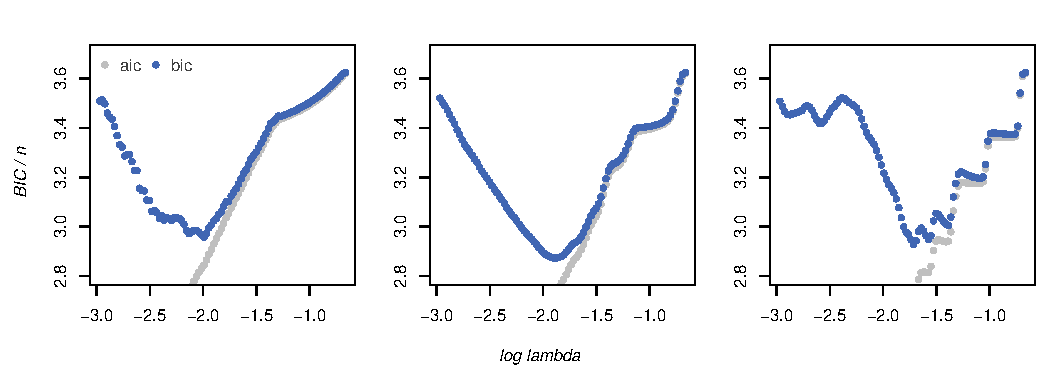
\includegraphics[width=6.3in]{../graphs/sim_ic}
\caption{\label{simic} BIC (with AIC in light gray) for our simulated linear regression example, on $\gamma = 0,2,10$. }

\vskip .7cm
{ \hskip 2.5cm$\bs{\gamma=0}$\hskip 4cm$\bs{\gamma=2}$\hskip 4cm$\bs{\gamma=10}$}
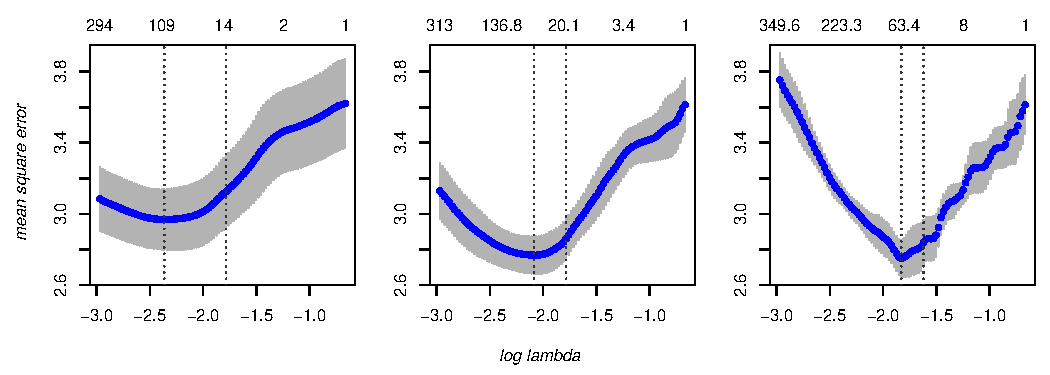
\includegraphics[width=6.3in]{../graphs/sim_cv}
\caption{\label{simcv} 5-fold CV results for our simulated data example. 
Points-and-bars show mean OOS deviance $\pm 1$se. Minimum and 1se selection rules are marked with dotted lines. }
\vspace{-.25cm}
\end{figure}


Figures \ref{simpaths} through \ref{simcv} illustrate an example analysis of
this data, with $n=1000$ and $p=2000$.  The paths are initialized at
$\lambda^1 = n^{-1}\max\{|g_j(\bm{0})|\}_{j=1}^p \approx 0.5$ as in Section \ref{glsec}, and each segment decreases as $\lambda^t
= \delta \lambda^{t-1}$ for $\delta=0.1^{\frac{1}{99}}$, through a grid of 100
values down to $\lambda^{100} \approx 0.05$. Coefficient penalties were divided by the corresponding covariate
standard deviation. 

The shapes of the regularization paths in Figure \ref{simpaths} show the
effect of increasing penalty concavity (via increasing $\gamma$), moving from
the lasso ($\gamma=0$) through the larger shoulders of $\gamma=2$ and on to
$\gamma=10$, where estimates move very quickly to the active-set MLE once a
variable is in-the-model.  Degrees of freedom, calculated as in (\ref{edf}),
are along the top of each plot; equal $\lambda$ have higher $df^t$ for higher
$\gamma$ since there is less shrinkage of $\hat\beta_j\neq0$.  The minimum BIC
model is marked upon each path plot with a vertical dashed line; it moves to
the right (higher $\lambda$) as $\gamma$ increases, selecting sparser models
under more concave penalties.


\begin{figure}[tbh] \vskip -.25cm { \hskip
2.5cm$\bs{\gamma=0}$\hskip 4cm$\bs{\gamma=2}$\hskip 4cm$\bs{\gamma=10}$}
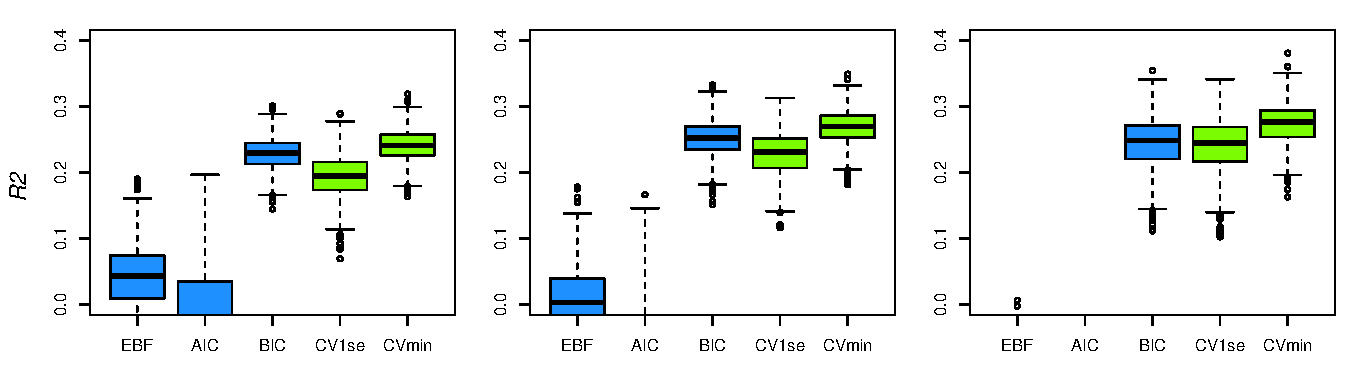
\includegraphics[width=6.3in]{../graphs/sim_oos} \caption{\label{simoos}
Out-of-sample simulation experiment results. } \end{figure}

AIC and BIC values along the paths are plotted in Figure \ref{simic}. Minimum
AIC models are not marked in Figure \ref{simpaths} because it always selected
the most complicated model.  The BIC curves resemble the 5-fold CV deviance
curves in Figure \ref{simcv}, and if one views OOS experiments as a gold-standard
 then this comparison favors BIC over AIC.  In Figure \ref{simcv},
dots mark mean OOS deviance and the bars spread $\pm$ 1 standard error for
this statistic.  The two CV selection rules, minimum-average  $\lambda_{\tt
min}$ (left vertical lines) and 1 standard error $\lambda_{\tt 1se}$ (right
vertical lines), are near each other and select similar models; both are
closer to the BIC than it is to the AIC.


A full comparison of selection methods and concavities is shown in Figure
\ref{simoos}, which evaluated fits on 1000 simulations from (\ref{simdgp}),
with $n=1000$ and $p=2000$, and their out-of-sample $R^2$ (one minus fitted
over null deviance) on another 1000 simulations of the same size.  For these
simulations we again use a grid of 100 segments, but smaller $\lambda^{100} =
0.01\lambda^1$.  BIC performs as well as CV, with $R^2$ falling between
$\lambda_{\tt min}$ (better) and $\lambda_{\tt 1se}$ (worse) rules.  The AIC
does far worse here, and actually selects models with majority negative OOS
$R^2$ for $\gamma >0$. We also show the EBF of \cite{zhou_path_2012}, which
does about as well as the AIC.\footnote{We use posterior MAP for
$\hat\sigma^2$ in the Zhou et al.~formulas.  Note that this is a
misapplication of the EBF procedure:  GL paths only approximate
minimization of the log penalized objective for which the EBF was derived.}

We do see a slight improvement in performance from $\gamma=0$ to $\gamma=2$:
10\% gain in average $R^2$ from 0.225 to 0.25 for BIC selected models
(significant given standard errors of about 8e-4). $\gamma=10$ also has higher
average $R^2$ (0.245 for BIC), but at the expense of more variation around the
mean. In some settings the performance gain will be larger and in others it
will be smaller. The benefits are probably not worth the trouble of full
optimization under a concave penalty, but may be enough to motivate the cheap
concavity offered by a gamma lasso with small $\gamma$.



\section{Hockey players}
\label{nhl}


\begin{figure}[p]
\vskip -1cm
\hskip -.5cm 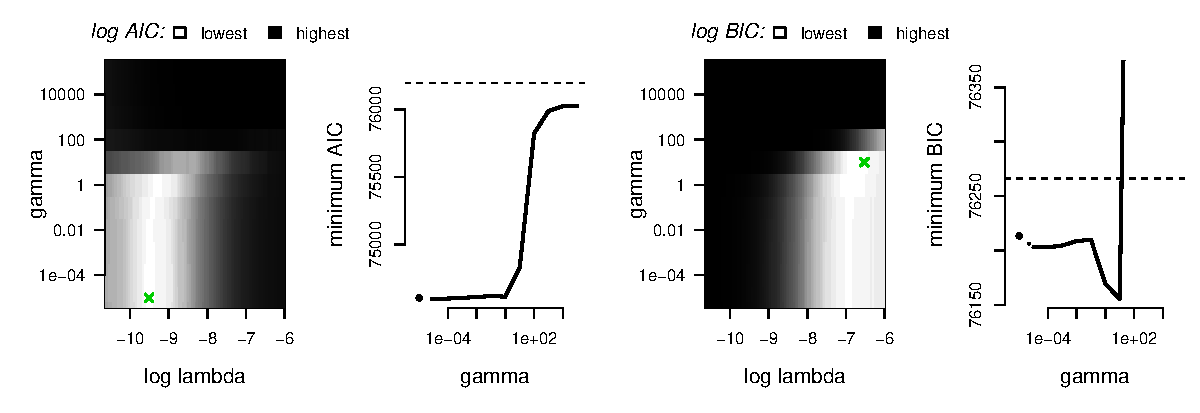
\includegraphics[width=6.5in]{../graphs/nhl_ic}
\caption{ \label{nhlic} Hockey example AIC and BIC for 
 100 $\log(\lambda)$ from -6 to -10.6 in models with  
 $\log_{10}\gamma = -5 \ldots 5$ and lasso $\gamma=0$.  `X' mark the 
 minima on the images, which have lasso on the bottom edge. Line plots show minimum IC across $\gamma$, with a dashed line for null model IC (with $\alpha$ and $\bs{\phi}$ only).
}

\vskip 1cm
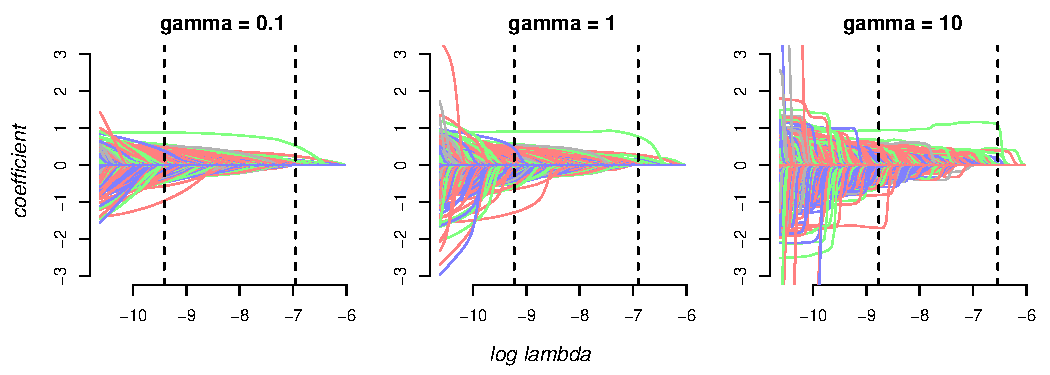
\includegraphics[width=6.4in]{../graphs/nhl_paths}
\caption{\label{nhlpaths} Hockey example regularization paths for 
$\gamma = 10^{\{-1,0,1\}}$; minimum AIC and BIC are marked with the dashed vertical lines.
Positions are shaded grey:goalie, blue:defense, green:center, red:winger.}

\vskip 1cm
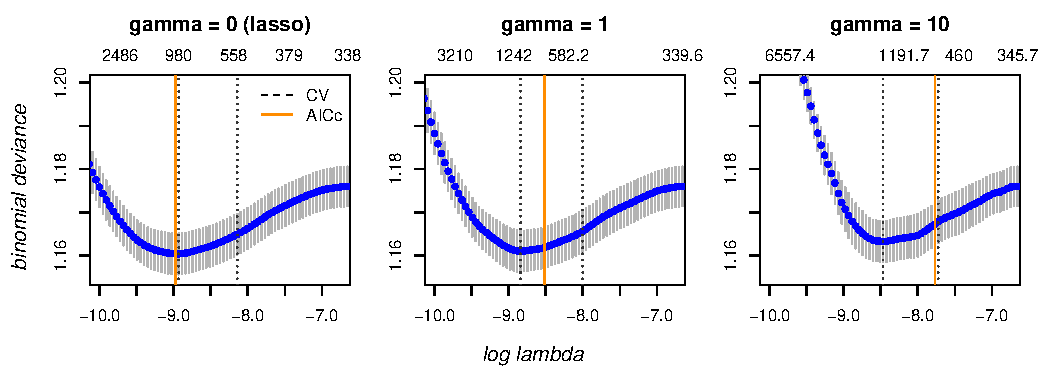
\includegraphics[width=6.4in]{../graphs/nhl_cv}
\caption{\label{nhlcv} Hockey example 20-fold CV: mean OOS deviance $\pm 1$se, with minimum and 1se selection rules marked with black dotted lines.  
Dashed (orange) lines show AIC and BIC selections. }
\end{figure}


Our next illustration investigates use of logistic regression to evaluate the
performance of hockey players.  This is an extension of the analysis in
\cite{gramacy_estimating_2013}.  The current version includes data about who
was on the ice for every goal in the National Hockey League (NHL) back to the
2002-2003 season, including playoffs.  The data
are in the {\tt gamlr} package for {\sf R}; there are
64540 goals and 2302 players.


Our `regression plus-minus' model for
player contribution is then, for goal $i$, 
\begin{align}\label{hockeymod}
\mr{logit}\left[\mr{p}(\text{home~team~scored~goal}~i)\right] = \alpha +
\bm{u}'\bs{\phi} + \bm{x}'\bs{\beta}, 
\end{align} 
where $\bm{u}$ is a length-7
vector of indicators for various special-teams scenarios (e.g., a home team
power play) and $\bm{x}$ is a vector of player effects: $x_{ij}=1$ if player
$j$ was on the home team and on ice for goal $i$, $x_{ij}=-1$ for away player
$j$ on ice for goal $i$, and $x_{ij}=0$ for everyone not on the ice.  
Thus the $\beta_j$ coefficients in (\ref{hockeymod}) correspond to the 
effect of an individual player on the log odds that, given a goal has been
scored, the goal was scored by their team.  This effect is `partial' in that
it controls for who else was on the ice (and special-teams
events)\footnote{Since goalies stay
on-ice for long periods (often entire games) their $\beta_j$  act as a
control for overall team quality.  Thus a skater (non-goalie) $\beta_j$ only need be
nonzero if that player is significantly above or below the team average.}, 
and since $\beta_j$ do not change from season
to season these are `career effects'.

We estimate gamma lasso paths of $\bs{\beta}$ for the model in
(\ref{hockeymod}), with  $\alpha$ and $\bs{\phi}$ left unpenalized, from  
$\lambda^1\approx \exp[-6]$ set as in (\ref{maxabsgrad}) down to $\lambda^{100} =
0.01\lambda^1$.  The penalties were {\it not} scaled by covariate standard
deviation, since this would have favored players with little ice time.  The
algorithm was run for $\log_{10}\gamma = -5 \ldots 5$, plus the $\gamma=0$
lasso.\footnote{On this data, $\gamma=\infty$ subset selection yields perfect separation and infinite likelihood.}
Joint $[\gamma,\lambda]$ surfaces
for AIC and BIC are in Figure \ref{nhlic}.  The BIC is minimized at higher $\lambda$
and $\gamma$ ($10$ and $e^{-6.5}$) than the AIC ($1^{-5}$ and $e^{-9.5}$), implying more sparsity but with less bias on
nonzero $\beta$.  Figure \ref{nhlic} also contains profiles
of BIC or AIC minima across $\gamma$: values are low for $\gamma \leq 1$,
but jump dramatically at 10 for the AIC and at 100 for the BIC (this is also the threshold start of higher compute times in Figure \ref{nhltime}).  
Figure \ref{nhlpaths}
shows paths on either side of $\gamma=1$, which appears to exist near a stability threshold: $\gamma\leq 1$ paths are smooth but for $\gamma=10$ the estimates jump from zero.

The low-BIC models for this data are very sparse.  At $\gamma=1$,
the BIC optimal
$\log(\lambda)=-6.9$
yields only 21 players with nonzero $\hat\beta_j$; these stars (all effects are positive) are shown in Figure
\ref{biceffects}.  This is due in large part to design multicollinearity:
since hockey players work on lines and are often matched against lines from
the opposing team, it is tough to isolate the performance of individuals.
With concave penalties imposing little bias on large signals, a few stars are assigned the
aggregate effect of their team-mates and common opponents.

The AIC  favors denser models with more bias.  The minimum-AIC lasso
($\gamma=0$) model identifies 904 nonzero player effects; the 20 largest (in
absolute value) are in Figure \ref{aiceffects}. Such estimates will be useful
to hockey analysts who wish to evaluate more than just a few key players.  The
increased bias also conforms to our prior expectation that single players
cannot have an overly large effect on the game. Indeed, the 20-fold CV results
in Figure \ref{nhlcv} support lower $\lambda$:  AIC selections are near the
minimum OOS deviance, and BIC selections are well to the right of the 1se OOS
deviance rule.  Comparing these results to those of Section \ref{sim}, where
the BIC was clearly superior, illustrates that no single model selection rule
is uniformly best.  Rather, AIC and BIC   provide informal bounds on model
complexity; use your knowledge of the application-at-hand (and OOS experiments
if possible) to make a final decision.


\begin{figure}[ht]

\vskip 1cm
{\footnotesize\sgl
\begin{verbatim}
  PETER_FORSBERG       MARIAN_HOSSA   PAVEL_DATSYUK       HENRIK_SEDIN 
           0.768              0.276           0.268              0.221 
NICKLAS_LIDSTROM        ZDENO_CHARA   SIDNEY_CROSBY  DANIEL_ALFREDSSON 
           0.137              0.134           0.115              0.114 
       DAN_BOYLE      NATHAN_HORTON    JOE_THORNTON     JONATHAN_TOEWS 
           0.114              0.097           0.092              0.085 
   ALEX_OVECHKIN       RYAN_GETZLAF    CHRIS_KUNITZ       JASON_ARNOTT 
           0.075              0.066           0.052              0.039 
    ALEX_TANGUAY VINCENT_LECAVALIER  MARIAN_GABORIK        ZACH_PARISE 
           0.036              0.033           0.019              0.015 
  ROBERTO_LUONGO 
           0.002 
\end{verbatim}}

\vskip -.5cm
\caption{\label{biceffects} All 21 non-zero player effects in the $\gamma = 1$ model at 
BIC optimal $\log(\lambda) = -6.9$.}

\vskip 1cm
{\footnotesize\sgl
\begin{verbatim}
NINO_NIEDERREITER   PETER_FORSBERG    RAITIS_IVANANS     BRAD_MARCHAND 
           -0.955            0.873            -0.568             0.560 
      PATRICK_ROY   MARTIN_GELINAS         ERIC_FEHR       THOMAS_POCK 
            0.511            0.488             0.486            -0.476 
 KENT_MANDERVILLE   JONATHAN_TOEWS      MARIAN_HOSSA   STEVEN_GOERTZEN 
           -0.471            0.466             0.453            -0.442 
    MATHIEU_BIRON    SIDNEY_CROSBY      RYAN_HOLLWEG        TIM_TAYLOR 
           -0.439            0.433            -0.430            -0.419 
   SCOTT_LACHANCE    PAVEL_DATSYUK   ALEXANDER_SEMIN      DALTON_PROUT 
           -0.418            0.416             0.408             0.407 
\end{verbatim}}

\vskip -.5cm \caption{\label{aiceffects} 20 largest player effects
(of 904 nonzero) in the lasso model at  AIC optimal $\log(\lambda) = -9.5$.
}

\end{figure}

\section{Discussion}
\label{discussion}

 We have found the gamma lasso
algorithm to be  useful and effective in application.  
Despite an abundance of theoretical and  empirical evidence showing that
concave penalties are superior to $L_1$ costs (for example,
see the references in Section \ref{lla}), our experience is that it is tough to do
{\it much} better than the simple lasso.  And it is easy to do worse.  The stable and fast gamma lasso algorithm provides an appealing middle
ground.

Despite our advocacy of the GL algorithm, this article was designed to be more of a review than an outline of new methods.  Our discussion finds that
the GL is very closely related to many different techniques in the dense
literature on concave regularization: it approximates MAP estimation of a
Bayesian model, or deviance minimization under log penalties, and is really
`just' a pathwise implementation of one-step LLA (or the adaptive lasso). A
central point of our review is that it is important to understand 
the entire regularization path (especially its continuity). This is especially
true under concave penalties, where due to multi-modality the solutions depend
(through hot-starts) on the route the path takes.  The point is made even
more explicit in GL estimation, where the size of the gap $\lambda^{t-1} -
\lambda^{t}$ changes the solution at $\lambda^t$.

Finally, any regularization path algorithm merely builds a set of candidate
models. Selection amongst these models is an essential extra step.  In our
case, we are selecting the `stopping point' $t$ and corresponding
$\bs{\hat\beta}^t$. Heuristic degrees of freedom for GL paths, and
resulting AIC/BIC metrics,  allow such selection through an intuitive
extension of lasso methods. CV is great, and easiest to
explain to non-statisticians, but it nice to have a fast analytic alternative.


\appendix

\section{Appendix}

\subsection{Gradient and curvature}
\label{models}

The
simplified negative log likelihood objective in Gaussian regression is $
l(\alpha,\bs{\beta}) = 0.5\sum_i (y_i -\eta_i)^2 $ with gradient
and coordinate curvature
\[
g_j(\bs{\beta}) = \frac{\partial l}{\partial \beta_j} = -\sum_i
x_{ij}(y_i - \eta_i),~~~~~~
h_j(\bs{\beta}) = \frac{\partial^2 l}{\partial \beta_j^2} = \sum_i
x_{ij}^2.
\]
In logistic regression, set $y_i = 1$ for `success' and $y_i = 0$ for
`failure' and write $q_i = (1 + \exp[-\eta_i])^{-1}$ as the
probability of success.  Then
$l(\alpha,\bs{\beta}) = \sum_i -y_i\eta_i + \log(1 +
  \exp[\eta_i])$ and
\[
g_j(\bs{\beta}) = \frac{\partial l}{\partial \beta_j} = -\sum_i
x_{ij}(y_i - q_i),~~~~~~
h_j(\bs{\beta}) = \frac{\partial^2 l}{\partial \beta_j^2} = \sum_i
x_{ij}^2q_i(1-q_i).
\]


% \subsection{Extra Proofs}

% It is
% straightforward to show that an appropriately weighted $L_1$ penalized
% deviance estimator will give predictions close to those from any such sparse
% approximation.  Our results are adapted from those in
% \citet{van_de_geer_adaptive_2011}.


% \begin{prop} Consider the weighted $L_1$ minimization from (\ref{l1pen}) in
% Algorithm 1, under squared-error loss $l(\hat\alpha,\bs{\hat\beta}) =
% \frac{1}{2}\|\bm{\hat y} - \bm{f} - \bs{\varepsilon}\|^2$.   Assume weights
% $\|\bs{\omega}_S\| = c_S\sqrt{s}/2$ and $\omega_j = 1$ $\forall j \in S^c$.
% Then for $\lambda$ large enough that $\max_j |\bs{x}_j'\bs{\varepsilon}| <
% n\lambda/4$, with $\bs{x}_j$ the $j^{th}$ design column, 
% \begin{equation} \frac{\|\bm{\hat y} - \bm{f}\|^2}{2n}\leq
% \frac{\|\bm{f}_S-\bm{f}\|^2}{n} +  \frac{3\lambda^2 (1+c_S)^2 s}{4\phi^2(2(1+c_S), s)}
% \end{equation} 
% where $\phi^2(L,s)$ is the restricted eigenvalue
% $
% \phi^2(L,s) = \min_{\{\bm{v}: |\bm{v}_{S^c}| \leq \sqrt{s}L\|\bm{v}_S\|\}}\bm{v}'\bs{\Sigma}\bm{v}
% $ defined on gram matrix $\bs{\Sigma} = \bm{X}'\bm{X}/n$.
% \end{prop}

% \begin{proof}
% This result is a direct adaptation of those in the book by \cite{buhlmann_statistics_2011}.

% \noindent We know that at convergence
% \[
% \|\bm{\hat y}-\bm{f}\|^2 - 2\bs{\varepsilon}'\bm{\hat y} + n\lambda\bs{\omega}'|\bs{\hat\beta}| \leq
% \|\bm{f}_S-\bm{f}\|^2 - 2\bs{\varepsilon}'\bm{f}_S + n\lambda\bs{\omega}_S'|\bs{\beta}_S|.
% \]
% By assumption $|\bs{\varepsilon}'\bs{x}_j|\leq n\lambda/4$ $\forall j$, so that $|\bs{\varepsilon}'\bm{\hat y}| = |\bs{\varepsilon}'\bm{X}\bs{\hat\beta}|
% \leq n\lambda|\bs{\hat\beta}_{S^c}|/4 + |\bs{\varepsilon}'\bm{X}_S\bs{\hat\beta}_S|$ and
% \begin{align*}
% \|\bm{\hat y}-\bm{f}\|^2 + \frac{n\lambda}{2}|\bs{\hat\beta}_{S^c}| &\leq 
% \|\bm{f}_S-\bm{f}\|^2 + |2\bs{\varepsilon}'\bm{X}_S (\bs{\hat\beta}_S - \bs{\beta}_S)| + n\lambda\bs{\omega}_S'|\bs{\hat\beta}_S - \bs{\beta}_S|\\
% &\leq \|\bm{f}_S-\bm{f}\|^2 + \frac{n\lambda}{2}|\bs{\hat\beta}_S - \bs{\beta}_S| + n\lambda\|\bs{\omega}_S\|\|\bs{\hat\beta}_S - \bs{\beta}_S\|\\
% &\leq \|\bm{f}_S-\bm{f}\|^2 + \frac{n\lambda\sqrt{s}}{2}\left(1+c_S\right)\|\bs{\hat\beta}_S - \bs{\beta}_S\|
% \end{align*}
% where we recall $c_S = 2\|\bs{\omega}_S\|/\sqrt{s}$.

% If $\|\bm{\hat y}-\bm{f}\|^2 + \frac{n\lambda}{2}|\bs{\hat\beta}_{S^c}|\leq2\|\bm{f}_S-\bm{f}\|^2 $ then we are done.  Otherwise,
% $\|\bm{\hat y}-\bm{f}\|^2 + \frac{n\lambda}{2}|\bs{\hat\beta}_{S^c}| <
% n\lambda \sqrt{s}\left(1+c_S\right)\|\bs{\hat\beta}_S - \bs{\beta}_S\|$.  By definition of the restricted eigenvalue, this yields $\|\bs{\hat\beta}_S - \bs{\beta}_S\| < 
% \|\bm{\hat y} - \bm{f}_S\|/[\sqrt{n}\phi(2(1+c_S),S)] < \left[\|\bm{\hat y} - \bm{f}\| + \|\bm{f}_S-\bm{f}\|\right]/[\sqrt{n}\phi(2(1+c_S),S)]$ and thus
% \begin{align*}
% \|\bm{\hat y}-\bm{f}\|^2 &\leq \frac{\sqrt{n}\lambda\sqrt{s}(1+c_S)}{\phi(2(1+c_S),S)}
% \left[\|\bm{\hat y} - \bm{f}\| + \|\bm{f}_S-\bm{f}\|\right] \\
% &\leq  \|\bm{f}_S-\bm{f}\|^2 + \frac{3n\lambda^2(1+c_S)^2s}{4\phi^2(2(1+c_S),S)} +
% \frac{\|\bm{\hat y}-\bm{f}\|^2}{2}
% \end{align*}
% since $0 \leq 2(\frac{a}{2}-c)^2 + (b-c)^2 = \frac{a^2}{2}+b^2+3c^2-2c(a+b)$ for any $a,b,c$.  
% \end{proof}


% \noindent {\bf Remarks}

% $\bullet$ For $j \in F=\hat S \cup S_\star^c$, the KKT conditions without any assumptions on irrepresentability imply
% \[
% 1 = \frac{1+\gamma\beta_j^{t-1}}{n\lambda_t}|\bs{x}_j'(\bm{\hat y} - \bm{f}-\varepsilon)|.
% \]
% Thus $n^2\lambda^2|F|^2/\|1+\gamma\beta_F^{t-1}\| < n^2\lambda^2\|\bs{\omega}_F\|$

\subsection{Sign Recovery}

\begin{theorem}\label{signrecov}
Under the setting of Theorem \ref{sparseapprox}, $\mr{sgn}(\bs{\hat\beta}) = \mr{sgn}(\bs{\beta}^\nu)$ for $\omega_{S^c}^{\mr{min}}\lambda > \sqrt{2\nu}$ if
\begin{equation}
\mr{(i)}~~|\bs{x}_j'\bm{X}_S(\bm{X}_S'\bm{X}_S)^{-1}\bs{\omega}_S| \leq 1 - \frac{\sqrt{2\nu}}{\lambda\omega_j}~~\forall~j ~\in~S^c
~~~
\mr{(ii)}~~\left|(\bm{X}_S'\bm{X}_S)^{-1}\bm{X}_S'\bm{y}\right|_\infty > n\lambda\left|(\bm{X}_S'\bm{X}_S)^{-1}\bs{\omega}_S\right|_\infty 
\end{equation}
\end{theorem}
\begin{proof} We adapt results of \cite{wainwright_sharp_2009}.
From the Karush-Kuhn-Tucker (KKT) conditions, 
$\bm{x}_j'\bm{X}(\bs{\hat\beta}_S-\bs{\beta}^\nu) + \bm{X}'\bm{e}^S = -n\lambda\zeta_j$ at convergence where $|\zeta_j| = \omega_j$ for $j\in\hat S$ and $|\zeta_j| \leq \omega_j$ for $j\in\hat S^c$.
Thus we we have no false positives if and only if
\begin{equation}
\bm{X}_S'\bm{X}_S(\bs{\hat\beta}_S-\bs{\beta}^\nu_S) + \bm{X}_S'\bm{e}^S =-n\lambda\bs{\zeta}_S ~~\Rightarrow~~ \bs{\hat\beta}_S-\bs{\beta}^\nu_S = -n\lambda(\bm{X}_S'\bm{X}_S)^{-1}\bs{\zeta}_S.
\end{equation}
And all of the spurious regressors in $S^c$ will have $\hat \beta_j = 0$
if and only if
\begin{equation}
\bs{x}_j'\bm{X}_S(\bs{\hat\beta}_S-\bs{\beta}^\nu_S) - \bs{x}_j'\bm{e}^S 
\leq n\lambda\zeta_j ~~\Leftarrow~~
1 - \frac{|x_j'\bm{e}^S|}{n} \geq 1 - \frac{\sqrt{2\nu}}{\lambda\omega_j} \geq |\bs{x}_j'\bm{X}_S(\bm{X}_S'\bm{X}_S)^{-1}\bs{\omega}_S|.
\end{equation}
Finally, for sign recovery on $j\in S$ we need 
\begin{equation}\label{signeq}
|\beta_j^\nu| - |\beta^\nu_j - \hat\beta_j| > 0 ~~\forall~j~\in~S,
\end{equation}
and $(ii)$ follows from  $\bs{\beta^\nu}_S = (\bm{X}_S'\bm{X}_S)^{-1}\bm{X}_S'\bm{y}$ and $ \bs{\beta^\nu}_S- \bs{\hat\beta}_S = n\lambda (\bm{X}_S'\bm{X}_S)^{-1}\bs{\zeta}_S$.

\end{proof}

\subsection{Quasi-Newton acceleration}
\label{qn}

Acceleration is applied to $\bs{\theta} = [\alpha,\bs{\beta}]$, the
set of both penalized and unpenalized parameters.  This move is
accepted only if it leads to a decrease in the objective,
such that there is no effect on algorithm convergence.
Suppose that $\bs{\hat\theta}^{(0)}$, $\bs{\hat\theta}^{(-1)}$, and
$\bs{\hat\theta}^{(-2)}$ are the current, previous, and
previous-to-previous parameter estimates.  Write
$M(\bs{\hat\theta}^{(t)})$ as the implied CD update map
$\bs{\hat\theta}^{(t)} \rightarrow \bs{\hat\theta}^{(t+1)}$, such that
the algorithm converges at $\bs{\hat\theta} - M(\bs{\hat\theta}) =
\bm{0}$.  With $\bm{u} = \bs{\hat\theta}^{(-1)} -
\bs{\hat\theta}^{(-2)}$ and $\bm{v} = \bs{\hat\theta}^{(0)} -
\bs{\hat\theta}^{(-1)}$, a secant approximation to the gradient of $M$
is $\partial M/\partial \hat\theta_l \approx \mr{v}_l/\mr{u}_l$.  An
approximate Newton-Raphson step to solve for the root of
$\bs{\hat\theta} - M(\bs{\hat\theta}) $  updates each
coordinate
\[
\hat \theta_l \gets
\hat\theta_l^{(-1)} - (\hat\theta_l^{(-1)} -
\hat\theta_l^{(0)})/(1-\mr{v}_l/\mr{u}_l)
\] which can be re-written as $\hat\theta_l =
(1-\mr{w}_l)\hat\theta_l^{(-1)} + \mr{w}_l\hat\theta_l^{(0)} $ where
$\mr{w}_l = \mr{u}_l/(\mr{u}_l - \mr{v}_l)$.


\sgl\small
\bibliographystyle{chicago}
\bibliography{gamlr}


\end{document}

